\documentclass[UTF8,twoside]{ctexart}

\usepackage{amsmath}
\usepackage{amssymb}
\usepackage{fancybox}
\usepackage{fancyhdr}
\usepackage{color}
\usepackage{bibentry}
\usepackage{multirow}
\usepackage[CJKbookmarks=true]{hyperref}
\usepackage{tikz}
\usepackage{mathrsfs}
\usepackage{bm}

\makeatletter % `@' now normal 'letter'
\@addtoreset{equation}{subsection}
\makeatother % `@' is restored as 'non-letter'
\makeatletter % `@' now normal 'letter'
\@addtoreset{figure}{section}
\makeatother % `@' is restored as 'non-letter'
\renewcommand\theequation{\oldstylenums{\thesubsection}%
.\oldstylenums{\arabic{equation}}}
\renewcommand\thefigure{\oldstylenums{\thesection}%
.\oldstylenums{\arabic{figure}}}

\DeclareMathOperator{\res}{Res}

\begin{document}
\setcounter{section}{4}
\title{现代量子力学}
\author{IRawaddy}

\maketitle
\thispagestyle{empty}

\pdfbookmark[1]{目录}{anchor}
\tableofcontents
\clearpage
\section{近似方法}

\noindent 在量子力学中,无论哈密顿量是不依赖于时间的还是依赖于时间的,都只有很少一部分问题可以被严格求解。因此我们不可避免地需要求助于某些近似形式。有些人认为,随着高速计算机的问世,我们总可以得到想要的数值解并达到足够的精确度;不过,在着手于富有野心的计算机运算前,理解近似解的物理基础依旧是很重要的事情。这一章我们将正当地系统探讨束缚态问题的近似解。

\subsection{不含时微扰理论:非简并情况}

\

\noindent \textbf{问题描述}

\noindent 我们在这里考虑的近似方法是不含时微扰理论,有时又叫做瑞利-薛定谔微扰理论。 我们考虑一个可以分成两部分的不含时哈密顿量$H$,换句话说,

\begin{equation} \label{5.1.1}
H = H_0 + V\text{,}
\end{equation}

\noindent 其中我们假定$V = 0$ 时的问题可以求出能量本征右矢$|n^{(0)}\rangle$ 和能量本征值$E_{n}^{(0)}$ 的严格解:

\begin{equation} \label{5.1.2}
H_0|n^{(0)}\rangle = E_{n}^{(0)}|n^{(0)}\rangle\text{。}
\end{equation}

\noindent 我们现在需要找到\emph{完整}哈密顿量所的近似本征右矢与本征值问题

\begin{equation} \label{5.1.3}
(H_0 + V)|n\rangle = E_n|n\rangle\text{,}
\end{equation}

\noindent 其中$V$被叫做扰动;通常情况下,它不是所有的势算符。比如,假设我们考虑氢原子在一个外部电场或磁场中。非微扰哈密顿量$H_0$由动能$\mathbf{p}^2/2m$ \emph{和}质子原子核的存在导致的库伦势$-e^2/r$ 组成。只有与外部$\mathbf{E}$ 或$\mathbf{B}$ 场作用而导致的势用扰动$V$来表示。

我们通常会求解下式来替代(\ref{5.1.3}):

\begin{equation} \label{5.1.4}
(H_0 + \lambda V)|n\rangle = E_n|n\rangle\text{,}
\end{equation}

\noindent 其中$\lambda$是一个连续实参量。引入这一参量是为了表示扰动被带入的倍数。在计算的最后我们可以让$\lambda \rightarrow 1$ 来回到完整倍数的扰动情况。换句话说,我们假定扰动的强度可以被调整。参量$\lambda$ 可以被想象成连续地从0 到1 变化,$\lambda = 0$ 对应于非微扰问题,而$\lambda = 1$对应于完整扰动强度的(\ref{5.1.3})。 在允许使用这种近似方法的物理情形下,我们希望当$\lambda$从0“调”到1时看到由$|n^0\rangle$ 到$n\rangle$和由$E_n^{(0)}$到$E_n$的转变为一个光滑过程。

这个方法依赖于能量本征值与能量本征右矢对于$\lambda$的幂展开。这意味着我们毫不怀疑的假设能量本征值与本征右矢在复$\lambda$-平面上$\lambda = 0$ 附近的解析性。当然,假如我们的方法只是为了实用兴趣,那么只要在展开中取前一到两项就可以得到很好的近似。


\noindent \textbf{双态问题}

\noindent 在我们着手于这一基本方法的系统表述前,先来看一下在我们已经遭遇多次的严格可解双态问题中,对$\lambda$ 的展开是如何确实有效的。假设我们有一哈密顿量可被写作

\begin{equation} \label{5.1.5}
H = E_{1}^{(0)}|1^{(0)}\rangle\langle1^{(0)}| + E_{2}^{(0)}|2^{(0)}\rangle\langle2^{(0)}| + \lambda V_{12}|1^{(0)}\rangle\langle 2^{(0)}| +  \lambda V_{21}|2^{(0)}\rangle\langle1^{(0)}|\text{,}
\end{equation}

\noindent 其中$|1^{(0)}\rangle$和$|2^{(0)}\rangle$是当$\lambda = 0$ 时的能量本征右矢,并且我们在此考虑$V_{11} = V_{22} = 0$。 这种表示下的$H$可以被描述为一个方阵:

\begin{equation} \label{5.1.6}
H = \left( \begin{array}{cc}
E_1^{(0)} & \lambda V_{12} \\
\lambda V_{21} & E_2^{(0)} \\
\end{array} \right)\text{,}
\end{equation}

\noindent 这里我们用到的是由非微扰本征右矢所组成的基底。显而易见地,矩阵$V$是厄米的;我们来求解$V_{12}$ 与$V_{21}$ 为实的情况:

\begin{equation} \label{5.1.7}
V_{12} = V_{21}^{\ast}\text{,}\quad V_{21}=V_{21}^{\ast}\text{;}
\end{equation}

\noindent 因此,由厄米性有

\begin{equation} \label{5.1.8}
V_{12} = V_{21}\text{。}
\end{equation}

\noindent 这一结果总可以通过调整$|2^{(0)}\rangle$相对于$|1^{(0)}\rangle$的相位来得到。这里求得能量本征值的过程与求解自旋取向问题完全类似,与(\ref{5.1.6})相似的有

\begin{equation} \label{5.1.9}
H = a_o + \boldsymbol{\sigma \cdot a} = \left( \begin{array}{cc}
a_0 + a_3 & a_1 \\
a_1 & a_0 - a_3 \\
\end{array} \right)\text{,}
\end{equation}

\noindent 这里我们假设$\boldsymbol{a} = (a_1,0,a_3)$很小且$a_0$,$a_1$,$a_3$都是实的。这一问题的本征值可知为

\begin{equation} \label{5.1.10}
E = a_0 \pm \sqrt{a_1^{2}+a_3^{2}}\text{。}
\end{equation}

\noindent 通过类比可得到对应于(\ref{5.1.6})的本征值为

\begin{equation} \label{5.1.11}
\left\{ \begin{array}{c}
E_1 \\
E_2 \\
\end{array} \right\} = \dfrac{\left(E_1^{\left(0\right)}+E_2^{\left(0\right)}\right)}{2}\pm \sqrt{\left[\dfrac{\left(E_1^{\left(0\right)} - E_2^{\left(0\right)}\right)^2}{4} + \lambda ^{2}|V_{12}|^{2} \right]}\text{。}
\end{equation}

\noindent 我们假设$\lambda|V_{12}|$相对于有关的能标,即非微扰能量本征值之差,是很小的:

\begin{equation} \label{5.1.12}
\lambda|V_{12}|\ll|E_1^{\left(0\right)}-E_2^{\left(0\right)}|\text{。}
\end{equation}

\noindent 我们便可以用

\begin{equation} \label{5.1.13}
\sqrt{1+\varepsilon} = 1 + \dfrac{1}{2}\varepsilon - \dfrac{\varepsilon ^2}{8} + \cdots
\end{equation}

\noindent 来得到在受到扰动$\lambda|V_{12}|$后能量本征值的展开,即,

\begin{equation} \label{5.1.14}
\begin{split}
&E_1 = E_1^{\left(0\right)} + \dfrac{\lambda^2|V_{12}|^2}{\left(E_1^{\left(0\right)} - E_2^{\left(0\right)}\right)} + \cdots \\
&E_2 = E_2^{\left(0\right)} + \dfrac{\lambda^2|V_{12}|^2}{\left(E_2^{\left(0\right)} - E_1^{\left(0\right)}\right)} + \cdots\text{。}
\end{split}
\end{equation}

\noindent 这就是可以通过刚才的到的一般形式轻而易举求得的表达式。我们同样可以类比自旋取向问题来写出能量本征右矢。

读者在这里可能被诱导着相信只要扰动足够弱就总是存在一个微扰展开。很不幸的是这并不是事实。作为一个基础例子,考虑一个质量为$m$的粒子被置于一个阱深$V_0$的极弱深方势阱中的一维问题(即当$-a< x< a$ 时$V = -V_0$,当$ |x|>a$ 时$V = 0$)。 这个问题允许一个束缚态能量,

\begin{equation} \label{5.1.15}
E = -(2ma^2/\hbar^2)|\lambda V|^2\text{,}\lambda>0\text{为吸引。}
\end{equation}

\noindent 我们可以将势阱看做一个加入自由粒子哈密顿量的极弱扰动并把结果(\ref{5.1.15})理解为从零到$|\lambda V|^2$ 的基态能移。 具体来说,由于(\ref{5.1.15}) 与$V$是二次相关的,我们可能有倾向地将其认为是通过二阶微扰理论所得到的基态能移。然而,这个观点是错的,因为假如事实真的如此,系统也会允许一个$E<0$ 的态对应于$\lambda$为负的排斥势,这完全是荒谬的。

现在我们来考察级数展开(\ref{5.1.14})的收敛半径。如果我们回头来看严格表示(\ref{5.1.11}) 并将其看做一个关于\emph{复变量}$\lambda$的方程,我们可以看出当$|\lambda|$ 从零开始增大时,会遇到枝点

\begin{equation} \label{5.1.16}
\lambda|V_{12}| = \dfrac{\pm i\left(E_1^{\left(0\right)}-E_2^{\left(0\right)}\right)}{2}\text{。}
\end{equation}

\noindent 当$\lambda=1$时的完整强度级数展开式的收敛条件为

\begin{equation} \label{5.1.17}
|V_{12}|<\dfrac{|E_1^{\left(0\right)}-E_2^{\left(0\right)}|}{2}\text{。}
\end{equation}

\noindent 如果这个条件不能被满足,那么微扰展开(\ref{5.1.14})就没有意义了。

\

\noindent \textbf{微扰展开进一步讨论}

现在我们对想要求解的基本问题引入更精确的表述。假如我们完全严格地知道

\begin{equation} \label{5.1.18}
H_0|n^{(0)}\rangle = E_n^{(0)}|n^{(0)}\rangle
\end{equation}

\noindent 的能量本征右矢和能量本征值。集合$\{|n^{(0)}\rangle\}$在满足闭合关系$1=\sum_n|n^{(0)}\rangle\langle n^{(0)}|$ 的意义下是完备的。 此外,我们假设这里的能谱是非简并的;在下一章我们会放宽这一假设。我们对于得到问题(\ref{5.1.4})的能量本征值与本征右矢很感兴趣。为了与(\ref{5.1.18}) 一致我们需要将(\ref{5.1.4}) 写为

\begin{equation} \label{5.1.19}
(H_0 + \lambda V)|n\rangle_\lambda = E_n^{(\lambda)}|n\rangle_\lambda
\end{equation}

\noindent 来表示能量本征值$E_n^{(\lambda)}$与能量本征右矢$|n\rangle_\lambda$是关于连续变化参量$\lambda$ 的函数;然而,我们将通常省略掉这些正确但又很累赘的角标。

由于连续参量$\lambda$是由0起增长的,我们希望第$n$个本征右矢的能量本征值$E_n$与其非微扰值$E_n^{(0)}$ 分离,所以我们定义第$n$ 级能移如下:

\begin{equation} \label{5.1.20}
\Delta_n\equiv E_n - E_n^{(0)}\text{。}
\end{equation}

\noindent 最基本要(近似)求解的薛定谔方程为

\begin{equation} \label{5.1.21}
(E_n^{(0)} - H_0)|n\rangle = (\lambda V - \Delta_n)|n\rangle\text{。}
\end{equation}

\noindent 我们可能倾向于对$E_n^{(0)} - H_0$算符取逆;然而,一般来说,逆算符$1/(E_n^{(0)} - H_0)$ 是定义不明的因为它可以作用于$|n^{(0)}\rangle$ 上。幸运的是在我们的问题中$(\lambda V - \Delta_n)|n\rangle$ 沿$|n^{(0)}\rangle$ 并没有分量,这可以通过在(\ref{5.1.21}) 两边左乘$\langle n^{(0)}|$ 来轻松得到:

\begin{equation} \label{5.1.22}
\langle n^{(0)}|(\lambda V - \Delta_n)|n \rangle = 0\text{。}
\end{equation}

\noindent 假如我们定义投影算子之补

\begin{equation} \label{5.1.23}
\phi_n\equiv 1-|n^{(0)}\rangle\langle n^{(0)}| =\displaystyle\sum_{k\neq n} |k^{(0)}\rangle\langle k^{(0)}|\text{。}
\end{equation}

\noindent 逆算符$1/(E_n^{(0)} - H_0)$在右乘$\phi_n$后就成了良好定义的。很明显,

\begin{equation} \label{5.1.24}
\dfrac{1}{E_n^{(0)}-H_0}\phi_n = \displaystyle\sum_{k\neq n}\dfrac{1}{E_n^{(0)}-E_k^{(0)}}|k^{(0)}\rangle\langle k^{(0)}|\text{。}
\end{equation}

\noindent 同样由(\ref{5.1.22})与(\ref{5.1.23}),显然有

\begin{equation} \label{5.1.25}
(\lambda V - \Delta_n)|n\rangle = \phi_n(\lambda V - \Delta_n)|n\rangle\text{。}
\end{equation}

\noindent 我们因此可能倾向于将(\ref{5.1.21})重新写为

\begin{equation} \label{5.1.26}
|n\rangle \overset{?}{=} \dfrac{1}{E_n^{(0)}-H_0}\phi_n(\lambda V-\Delta_n)|n\rangle\text{。}
\end{equation}

\noindent 然而,这不可能是正确的因为在$\lambda \rightarrow 0$时,我们必须得到$|n\rangle \rightarrow |n^{(0)}\rangle$ 和$\Delta_n \rightarrow 0$。然而,即使$\lambda \neq 0$ ,我们也总可以给$|n\rangle$ 添加一个齐次方程(\ref{5.1.18}) 的解,即,$c_n|n^{(0)}\rangle$,因此一个更合适的最终形式是

\begin{equation} \label{5.1.27}
|n\rangle = c_n(\lambda)|n^{(0)}\rangle + \dfrac{1}{E_n^{(0)}-H_0}\phi_n(\lambda V - \Delta_n)|n\rangle\text{,}
\end{equation}

\noindent 其中

\begin{equation} \label{5.1.28}
\lim\limits_{\lambda \to 0}c_n(\lambda) = 1\text{。}
\end{equation}

\noindent 注意到

\begin{equation} \label{5.1.29}
c_n(\lambda) = \langle n^{(0)}|n\rangle\text{。}
\end{equation}

\noindent 由于我们接下来将要说明的原因,舍弃常用的归一化约定是很方便的

\begin{equation} \label{5.1.30}
\langle n|n\rangle = 1\text{。}
\end{equation}

\noindent 某种程度上,我们令

\begin{equation} \label{5.1.31}
\langle n^{(0)}|n\rangle = c_n(\lambda) = 1\text{,}
\end{equation}

\noindent 即使是$\lambda \neq 0$。只要我们不在意整体的归一化我们便总是可以这样做因为令$c_n\neq 1$ 的唯一影响只是引入一个公因子。因此,如果愿意,我们总可以在计算的最后再将右矢归一化。习惯上我们也会写

\begin{equation} \label{5.1.32}
\dfrac{1}{E_n^{(0)}-H_0}\phi_n \rightarrow \dfrac{\phi_n}{E_n^{(0)}-H_0}
\end{equation}

\noindent 和

\begin{equation} \label{5.1.33}
\dfrac{1}{E_n^{(0)}-H_0}\phi_n = \phi_n\dfrac{1}{E_n^{(0)}-H_0} = \phi_n\dfrac{1}{E_n^{(0)}-H_0}\phi_n\text{,}
\end{equation}

\noindent 因此我们有

\begin{equation} \label{5.1.34}
|n\rangle=|n^{(0)}\rangle + \dfrac{\phi_n}{E_n^{(0)}-H_0}(\lambda V-\Delta_n)|n\rangle\text{。}
\end{equation}

\noindent 我们还注意到由(\ref{5.1.22})与(\ref{5.1.31})有

\begin{equation} \label{5.1.35}
\Delta_n = \lambda \langle n^{(0)}|V|n\rangle\text{。}
\end{equation}

任何过程都基于(\ref{5.1.34})和(\ref{5.1.35})这两个等式。我们的基本策略是将$|n\rangle$ 和$\Delta_n$ 展开到$\lambda$ 的幂再匹配适当的系数。这是合理的因为(\ref{5.1.34}) 与(\ref{5.1.35})是两个对$\lambda$从0到1 取值恒成立的等式。 我们在最开始写出

\begin{equation} \label{5.1.36}
\begin{split}
&|n\rangle = |n^{(0)}\rangle + \lambda|n^{(1)}\rangle + \lambda^2|n^{(2)}\rangle + \cdots \\
&\Delta_n = \lambda\Delta_n^{(1)} + \lambda^2\Delta_n^{(2)} + \cdots\text{。}
\end{split}
\end{equation}

\noindent 将(\ref{5.1.36})代入(\ref{5.1.35})并取$\lambda$各次幂对应的系数相等,我们可以得到

\begin{equation} \label{5.1.37}
\begin{array}{cccc}
O(\lambda^1): & \Delta_n^{(1)} & = & \langle n^{(0)}|V|n^{(0)}\rangle  \\
O(\lambda^2): & \Delta_n^{(2)} & = & \langle n^{(0)}|V|n^{(1)}\rangle  \\
\vdots & \quad & \vdots & \quad \\
O(\lambda^N): & \Delta_n^{(N)} & = & \langle n^{(0)}|V|n^{(N-1)}\rangle\text{,}  \\
\vdots & \quad & \vdots & \quad
\end{array}
\end{equation}

\noindent 因此想要求出$\lambda^N$阶的能移只需要知道到$\lambda^{N-1}$ 阶的$|n\rangle$。 我们现在来看(\ref{5.1.34});当用(\ref{5.1.36}) 对其展开时,我们得到

\begin{equation} \label{5.1.38}
\begin{split}
|n^{(0)}\rangle + &\lambda|n^{(1)}\rangle + \lambda^2|n^{(2)}\rangle + \cdots \\
= &|n^{(0)}\rangle + \dfrac{\phi_n}{E_n^{(0)}-H_0}(\lambda V - \lambda\Delta_n^{(1)} - \lambda^2\Delta_n^{(2)} - \cdots) \\
&\times(|n^{(0)}\rangle + \lambda|n^{(1)}\rangle+\cdots)\text{。}
\end{split}
\end{equation}

\noindent 取$\lambda$各次幂对应的系数相等,我们便有

\begin{equation} \label{5.1.39}
O(\lambda):\quad|n^{(1)}\rangle = \dfrac{\phi_n}{E_n^{(0)}-H_0}V|n^{(0)}\rangle\text{,}
\end{equation}

\noindent 这里我们用到了$\phi_n\Delta_n^{(1)}|n^{(0)}\rangle = 0$。有了$|n^{(1)}\rangle$后,回头再来看我们先前得到的$\Delta_n^{(2)}$的表达式[见(\ref{5.1.37})]就有价值了:

\begin{equation} \label{5.1.40}
\Delta_n^{(2)} = \langle n^{(0)}|V\dfrac{\phi_n}{E_n^{(0)}-H_0}V|n^{(0)}\rangle\text{。}
\end{equation}

\noindent 知道了$\Delta_n^{(2)}$,我们便能同样运用(\ref{5.1.39})得到右矢方程\ref{5.1.38}) 中的$\lambda^2-$ 项如下:

\begin{equation} \label{5.1.41}
\begin{split}
O(\lambda^2):\quad |n^{(2)}\rangle = &\dfrac{\phi_n}{E_n^{(0)}-H_0}V\dfrac{\phi_n}{E_n^{(0)}-H_0}V|n^{(0)}\rangle \\
&-\dfrac{\phi_n}{E_n^{(0)}-H_0}\langle n^{(0)}|V|n^{(0)}\rangle\dfrac{\phi_n}{E_n^{(0)}-H_0}V|n^{(0)}\rangle\text{。}
\end{split}
\end{equation}

\noindent 很明显,只要我们想便可以继续这种模式。我们的算符研究方法相当简洁;我们不用每次都把指数写出来。当然,在实际运算中我们需要在最后使用(\ref{5.1.23})所给出的$\phi_n$的具体形式。

为了看出这些究竟怎样奏效,我们写出能移的具体展开

\begin{equation} \label{5.1.42}
\Delta_n \equiv E_n-E_n{(0)} \\
= \lambda V_{nn} + \lambda^2 \displaystyle\sum_{k\neq n}\dfrac {|V_{nk}|^2}{E_n^{(0)}-E_k^{(0)}} + \cdots\text{,}
\end{equation}

\noindent 其中

\begin{equation} \label{5.1.43}
V_{nk} \equiv \langle n^{(0)}|V|k^{(0)}\rangle \neq \langle n|V|k\rangle\text{,}
\end{equation}

\noindent 也就是,矩阵元是依赖于\emph{非微扰}右矢的。注意到当我们对双态问题进行展开时我们便重新得到了先前(\ref{5.1.14})的表达式。微扰右矢的展开如下:

\begin{equation} \label{5.1.44}
\begin{split}
|n\rangle = &|n^{(0)}\rangle + \lambda\displaystyle\sum_{k\neq n}|k^{(0)}\rangle\dfrac{V_{kn}}{E_n^{(0)}-E_k^{(0)}} \\
&+ \lambda^2 \left(\displaystyle\sum_{k\neq n}\displaystyle\sum_{l\neq n}\dfrac{|k^{(0)}\rangle V_{kl}V_{ln}}{(E_n^{(0)}-E_k^{(0)})(E_n^{(0)}-E_l^{(0)})}-\displaystyle\sum_{k\neq n}\dfrac{|k^{(0)}\rangle V_{nn}V_{kn}}{(E_n^{(0)}-E_k^{(0)})^2}\right) \\
&+ \cdots\text{。}
\end{split}
\end{equation}

\noindent 方程(\ref{5.1.44})表明第$n$能级不再与非微扰右矢$|n^{(0)}\rangle$ 成正比而是含有其他的非微扰能量右矢;换句话说,扰动$V$混合了多个非微扰能量本征右矢。

一些普遍的要点依序如下。第一,想取得一阶能移需要求出$V$关于非微扰右矢的期望值。第二,由二阶能移的展开(\ref{5.1.42})不难看出两个能级,设为第$i$ 和$j$ 能级,通过$V_{ij}$共同作用时会趋向于互相排斥;低一些的能级,设为第$i$ 级,由于与更高的$j$ 能级混合会趋于降低$|V_{ij}|^2/(E_j^{(0)}-E_i^{(0)})$,同时$j$ 级的能量会提升相同的数值。这是{\textbf{能级互不交叉定理}}的一个特例,它表明一对能级受扰动共同影响时不会随扰动强度的变动而产生交叉。

假定这里有不止一对能级有可知的矩阵元但右矢$|n\rangle$,即我们关心其能量的那一个,依赖于基态;那么(\ref{5.1.42}) 中关于二阶能移的每一项都是负的。这意味着基态的二阶能移永远是负的;由于混合的结果导致最低态趋向于变得更低。

很明显如果$|V_{il}/(E_i^{(0)}-E_l^{(0)})|$足够“小”那么微扰展开(\ref{5.1.42}) 和(\ref{5.1.44}) 都将收敛。一个更加精确的判断可以在$H_0$仅为动能算符时给出(此时的瑞利- 薛定谔微扰展开就仅变成了波恩级数) :当能量$E_0<0$ ,波恩级数收敛当且仅当$H_0+V$ 与$H_0-V$ 都没有束缚态能量使$E\leq E_0$ 。见Newton(1982),p.233。

\noindent \textbf{波函数的重整化}

\noindent 我们现在能够探究微扰右矢的归一化了。考虑我们用的归一化约定,(\ref{5.1.31}),我们看出微扰右矢$|n\rangle$ 在通常样式下不是被归一化的。我们可以通过定义

\begin{equation} \label{5.1.45}
|n\rangle_N = Z_n^{1/2}|n\rangle
\end{equation}

\noindent 来将微扰右矢重整化,其中$Z_n$是一个常数有$\phantom{\rangle}_N\langle n|n\rangle_N = 1$。左乘$\langle n^{(0)}|$我们便可以[由(\ref{5.1.31})]得到

\begin{equation} \label{5.1.46}
Z_n^{1/2} = \langle n^{(0)}|n\rangle_N\text{。}
\end{equation}

\noindent $Z_n$的物理意义是什么?因为$|n\rangle_N$满足一般的归一化要求(\ref{5.1.30}) ,$Z_n$ 可以被当做在对应的非微扰能量本征态中找到微扰能量本征态的概率。注意到

\begin{equation} \label{5.1.47}
\phantom{\rangle}_N\langle n|n\rangle_N = Z_n\langle n|n\rangle = 1\text{,}
\end{equation}

\noindent 我们有

\begin{subequations} \label{5.1.48a}
\begin{align}
\begin{split}
Z_n^{-1} = &\langle n|n\rangle = (\langle n^{(0)}|+\lambda \langle n^{(1)}| + \lambda^2 \langle n^{(2)}| + \cdots)\\
&\times(|n^{(0)}\rangle + \lambda|n^{(1)}\rangle + \lambda^2|n^{(2)}\rangle + \cdots)\\
=& 1 + \lambda^2\langle n^{(1)}|n^{(1)}\rangle + O(\lambda^3) \\
=& 1 + \lambda^2\displaystyle\sum_{k\neq n}\dfrac{|V_{kn}|^2}{\left(E_n^{(0)}-E_k^{(0)}\right)^2} + O(\lambda^3)\text{,}
\end{split}
\end{align}
\noindent 因此取到$\lambda^2$阶,我们便得到了在对应的非微扰态中找到微扰态的概率

\begin{align}\label{5.1.48b}
 Z_n\backsimeq 1-\lambda^2\displaystyle\sum_{k\neq n}\dfrac{|V_{kn}|^2}{\left(E_n^{(0)}-E_k^{(0)}\right)^2}\text{。}
\end{align}
\end{subequations}

\noindent (\ref{5.1.48b})中的第二项可以当做向$|n^{(0)}\rangle$ 以外的态“泄露”的概率。注意到$Z_n$ 是小于1 的,这正好符合了将$Z$认定为概率的基本诠释。

有趣的是我们从(\ref{5.1.42})中注意到对于$\lambda^2$阶,$Z$ 和$E_n$ 对$E_n^{(0)}$ 导数有直接关系如下:

\begin{equation} \label{5.1.49}
Z_n = \dfrac{\partial E_n}{\partial E_n^{(0)}}\text{。}
\end{equation}

\noindent 当然,我们明白在取$E_n$对$E_n^{(0)}$偏导数的过程中,我们必须将$V$ 的矩阵元看做固定量。结论(\ref{5.1.49}) 实际上相当普适且不仅局限于二阶微扰理论。

\noindent \textbf{基本例子}

\noindent 为了举例说明我们发展后的微扰方法,我们来看两个例子。首先考虑一个简谐振子其非微扰哈密顿量即通常形式:

\begin{equation} \label{5.1.50}
H_0 = \dfrac{p^2}{2m} + \dfrac{1}{2}m\omega^2 x^2\text{。}
\end{equation}

\noindent 假设弹簧弹性系数$k=m\omega^2$在轻微变动。我们可以将其变更表示为增加一个额外的势

\begin{equation} \label{5.1.51}
V = \dfrac{1}{2}\varepsilon m\omega^2 x^2\text{,}
\end{equation}

\noindent 其中$\varepsilon$是一个满足$\varepsilon \ll 1$的无量纲常数。某种观点来看,这个问题太简单了根本不需要用围绕理论;我们只要对$\omega$ 做如下变化即可马上得到严格解:

\begin{equation} \label{5.1.52}
\omega \rightarrow \sqrt{1+\varepsilon}\omega\text{,}
\end{equation}

\noindent 然而这是一个有教育意义的例子因为他提供了微扰近似与严格解法之间的比较。

我们现在关注的是在存在$V$时的新基态右矢$|0\rangle$以及基态能移$\Delta_0$:

\begin{subequations} \label{5.1.53a}
\begin{align}
|0\rangle = |0^{(0)}\rangle + \displaystyle\sum_{k\neq0}|k^{(0)}\rangle\dfrac{V_{k0}}{E_0^{(0)}-E_k^{(0)}}+\cdots
\end{align}
 \noindent 以及
\begin{align} \label{5.1.53b}
\Delta_0 = V_{00} + \displaystyle\sum_{k\neq0}\dfrac{|V_{k0}|^2}{E_0^{(0)}-E_k^{(0)}}+\cdots\text{。}
\end{align}
\end{subequations}

\noindent 这里相应的矩阵元为(参见本章问题5)

\begin{equation} \label{5.1.54}
\begin{split}
&V_{00}=\left(\dfrac{\varepsilon m\omega^2}{2}\right)\langle0^{(0)}|x^2|0^{(0)}\rangle=\dfrac{\varepsilon\hbar\omega}{4} \\
&V_{20}=\left(\dfrac{\varepsilon m\omega^2}{2}\right)\langle2^{(0)}|x^2|0^{(0)}\rangle=\dfrac{\varepsilon\hbar\omega}{2\sqrt{2}}\text{。}
\end{split}
\end{equation}

\noindent 其他$V_{k0}$形式的矩阵元为零。注意到(\ref{5.1.53a})与(\ref{5.1.53b})中的非零能量分母是$-2\hbar\omega$,我们可以结合现有结果来得到

\begin{subequations} \label{5.1.55a}
\begin{align}
|0\rangle=|0^{(0)}\rangle-\dfrac{\varepsilon}{4\sqrt{2}}|2^{(0)}\rangle+O(\varepsilon^2)
\end{align}
 \noindent 和
\begin{align} \label{5.1.55b}
\Delta_0=E_0-E_0^{(0)}=\hbar\omega\left[\dfrac{\varepsilon}{4}-\dfrac{\varepsilon^2}{16}+O(\varepsilon^3)\right]\text{。}
\end{align}
\end{subequations}

\noindent 注意到由于微扰,基态右矢在展开成原有非微扰能量本征右矢$\{|n^{(0)}\rangle\}$的项后,会出现一个沿第二激发态方向的分量。沿第一激发态方向分量的缺失并不令人感到奇怪因为我们的\emph{总}$H$ 是宇称不变的;因此,一个能量本征态也被期望是宇称本征态。

对于能移而言的与严格方法的对比可以轻松获得如下:

\begin{equation} \label{5.1.56}
\dfrac{\hbar\omega}{2} \rightarrow \left(\dfrac{\hbar\omega}{2}\right)\sqrt{1+\varepsilon} = \left(\dfrac{\hbar\omega}{2}\right)\left[1+\dfrac{\varepsilon}{2}-\dfrac{\varepsilon^2}{8}+\cdots\right] \text{,}
\end{equation}

\noindent 与(\ref{5.1.55b})完全一致。对于微扰右矢,我们观察波函数的变化。在没有$V$ 时基态波函数为

\begin{equation} \label{5.1.57}
\langle x|0^{(0)}\rangle = \dfrac{1}{\pi^{1/4}}\dfrac{1}{\sqrt{x_0}}e^{-x^2/2x_0^2}\text{,}
\end{equation}

\noindent 其中

\begin{equation} \label{5.1.58}
x_0\equiv\displaystyle\sqrt{\dfrac{\hbar}{m\omega}}\text{。}
\end{equation}

\noindent 代入(\ref{5.1.52})便得到

\begin{equation} \label{5.1.59}
x_0 \rightarrow \dfrac{x_0}{(1+\varepsilon)^{1/4}}\text{;}
\end{equation}

\noindent 因此,

\begin{equation} \label{5.1.60}
\begin{split}
\langle x|0^{(0)}\rangle&\rightarrow\dfrac{1}{\pi^{1/4}\sqrt{x_0}}(1 + \varepsilon)^{1/8}\exp\left[-\left(\dfrac{x^2}{2x_0^2}\right)(1+\varepsilon)^{1/2}\right]\\
&\simeq\dfrac{1}{\pi^{1/4}}\dfrac{1}{\sqrt{x_0}}e^{-x^2/2x_0^2}+ \dfrac{\varepsilon}{\pi^{1/4}\sqrt{x_0}} e^{-x^2/2x_0^2}\left[\dfrac{1}{8}-\dfrac{1}{4}\dfrac{x^2}{x_0^2}\right] \\
& = \langle x|0^{(0)}\rangle-\dfrac{\varepsilon}{4\sqrt{2}}\langle x|2^{(0)}\rangle\text{,}
\end{split}
\end{equation}

\noindent 这里我们用到了

\begin{equation} \label{5.1.61}
\begin{split}
\langle x|2^{(0)}\rangle &= \dfrac{1}{2\sqrt{2}}\langle x|0^{(0)}\rangle H_2\left(\dfrac{x}{x_0}\right) \\
&= \dfrac{1}{2\sqrt{2}}\dfrac{1}{\pi^{1/4}}\dfrac{1}{\sqrt{x_0}}e^{-x^2/2x_0^2} \left[-2+4\left(\dfrac{x}{x_0}\right)^2\right]\text{,}
\end{split}
\end{equation}

\noindent 以及$H_2(x/x_0)$是一个二阶厄米多项式。

作为非简并微扰理论的示例,我们讨论{\textbf{二次斯塔克效应}}。一个单电子原子,如氢原子或者在(球对称)满壳层外拥有一个价电子的类氢原子,被放入一个沿$z$-轴正方向的固定电场中。哈密顿量$H$可以被分为两部分,

\begin{equation} \label{5.1.62}
H_0=\dfrac{\boldsymbol{p}^2}{2m}+V_0(r)\quad \text{其中} \quad V=-e|{\boldsymbol{E}}|z\quad(\text{对于电子}e<0)
\end{equation}

\noindent [编者注:由于当$z\rightarrow -\infty$时扰动$V\rightarrow -\infty$,当然,由$H_0$ 束缚的粒子现在可以逃逸,而且原先所有的束缚态便只有一个有限的持续时间。然而,我们依然可以形式地用微扰理论来计算能移。(这个位移的虚部,在此处会被省略,它可以给出态的持续时间或对应的共振宽度。)]

这里假设非微扰(只有$H_0$)的能量本征右矢与能谱都是完全知道的。电子自旋被证实与问题并不相干,而且我们假设忽略自旋自由度后,没有能级是简并的。这个假设不符合氢原子的$n\neq 1$能级,其中$V_0$是纯库伦势;我们将晚些讨论这一问题。能移写作

\begin{equation} \label{5.1.63}
\Delta_k=-e|{\boldsymbol{E}}|z_{kk}+e^2|{\boldsymbol{E}}|^2\displaystyle\sum_{j\neq k} \dfrac{|z_{kj}|^2}{E_k^{(0)}-E_j^{(0)}}+\cdots\text{,}
\end{equation}

\noindent 其中我们用$k$来取代$n$以避免与主量子数$n$产生混淆。由于没有简并度,$|k^{(0)}\rangle$ 被预期为宇称本征态;因此

\begin{equation} \label{5.1.64}
z_{kk}=0\text{,}
\end{equation}

\noindent 正如我们在4.2节所看到的。物理角度来说,此处不会有线性斯塔克效应,即,因为原子具有一个为零的永电偶极子所以能移中不会有与$|{\boldsymbol{E}}|$成正比的项,因此能移在$e^3|{\boldsymbol{E}}^3|$ 或更高阶项被忽略的情况下与$|{\boldsymbol{E}}|$ 是二次相关的。

我们现在来注意$z_{kj}$,它出现在(\ref{5.1.63}),其中$k$(或$j$)是用来代表$(n,l,m)$和$(n^{\prime} ,l^{\prime} ,m^{\prime})$的\textbf{指标集}。首先,我们来重提选择定理[见(\ref{3.11.39})]

\begin{equation} \label{5.1.65}
\langle n^{\prime},l^{\prime}m^{\prime}|z|n,lm\rangle=0 \quad \text{除非} \Big\{\begin{array}{l}
l^{\prime}=l\pm 1 \\
m^{\prime}=m
\end{array}
\end{equation}

\noindent 其由对角动量($T_{q=0}^{(1)}$的维格纳-埃卡特定理)和宇称的考量而得到的。

这里有另一种方式来看待$m$-选择定理。在存在$V$的情况下,哈密顿量的完整球对称性被沿$z$- 轴正方向的外加电场所破坏,但是$V$(因此也有完整的$H$)在绕$z$-轴转动时是不变的;换句话说,我们还有柱对称性。正式来说这可以由事实

\begin{equation} \label{5.1.66}
[V,L_z]=0
\end{equation}

\noindent 来反映。这意味着$L_z$即便在存在$V$的情况下依旧是好量子数。因此,扰动可以被写作具有相同的$m$ 的$L_z$ 本征右矢的叠加,这个问题中即$m=0$。这一说法对于所有阶都成立,尤其是,对于一阶右矢。而且,因为二阶能移是由一阶右矢所得的[见(\ref{5.1.40})],我们便可明白为什么只有$m=0$的项对求和有贡献。

原子的极化率$\alpha$由原子态的能移定义如下:
\begin{equation} \label{5.1.67}
\Delta=-\dfrac{1}{2}\alpha|{\boldsymbol{E}}|^2\text{。}
\end{equation}

\noindent 我们来考虑氢原子基态这一特殊情况。尽管氢原子激发态的能谱是简并的,但是基态(在忽略自旋时)是非简并的,因此非简并微扰理论的方法可以运用的。基态$|0^{(0)}\rangle$ 用$(n,l,m)$ 指标表示是$(1,0,0)$,因此

\begin{equation} \label{5.1.68}
\alpha=-2e^2\displaystyle\sum_{k\neq0}^{\infty}\dfrac{|\langle k^{(0)}|z|1,0,0\rangle|^2}{\left[E_0^{(0)}-E_k^{(0)}\right]}\text{,}
\end{equation}

\noindent  其中针对$k$的求和不但包含了所有束缚态$|n,l,m\rangle$(其中n>1),还包含了氢原子的正能量连续态。

这里有很多办法来通过多种繁杂度来近似估计或严格求解(\ref{5.1.68})中的求和。我们在此展示最简单的方法。假设(\ref{5.1.68}) 中的分母都是常数。 这样我们就可以通过考虑

\begin{equation} \label{5.1.69}
\begin{split}
\displaystyle\sum_{k\neq0}|\langle k^{(0)}|z|1,0,0\rangle|^2 &= \sum_{\text{所有} k}|\langle k^{(0)}|z|1,0,0\rangle|^2\\
& =\langle1,0,0|z^2|1,0,0\rangle
\end{split}
\end{equation}

\noindent 来得到求和,其中我们在最后一步运用了完备性关系。但我们可以轻松地对基态的$\langle z^2\rangle$ 求值如下:

\begin{equation} \label{5.1.70}
\langle z^2\rangle=\langle x^2\rangle=\langle y^2\rangle=\dfrac{1}{3}\langle r^2\rangle\text{,}
\end{equation}

\noindent 其次通过运用波函数的准确形式可以得到

\begin{equation}
\langle r^2\rangle=a_0^2\text{,}
\end{equation}

\noindent 其中$a_0$表示玻尔半径。很不幸的是极化率$\alpha$的表示中存在依赖于$E_k^{(0)}$ 的能量分母,但是我们知道不等式

\begin{equation} \label{5.1.71}
-E_0^{(0)}+E_k^{(0)}\geq -E_0^{(0)}+E_1^{(0)}=\dfrac{e^2}{2a_0}\left[1-\dfrac{1}{4}\right]
\end{equation}

\noindent 适用于(\ref{5.1.68})中的任何能量分母。因此,我们可以得到氢原子基态极化率的一个上限,即,

\begin{equation} \label{5.1.72}
\alpha<\dfrac{16a_0^3}{3}\simeq5.3a_0^3\text{,}
\end{equation}

\noindent 值得一提的是我们可以用A·Dalgarno与J·T·Lewis提出的方法(如Merzbacher 1970,p.424)来严格求得(\ref{5.1.68}) 中的求和,这同样与实践测量相符。这给出

\begin{equation} \label{5.1.73}
\alpha=\dfrac{9a_0^3}{2}=4.5a_0^3\text{。}
\end{equation}

\noindent 我们可以(不运用微扰理论)通过使用双曲坐标求解薛定谔方程来得到完全相同的解。

\subsection{不含时微扰理论:简并情况}

\

\noindent 我们前一节中所发展的微扰方法在遇到非微扰能量本征右矢简并是会失效。上一节的方法是假设有一个唯一且良好定义的能量$E_n^{(0)}$的非微扰右矢使得微扰右矢在$\lambda\rightarrow0$时趋近。然而,当简并存在时,任何由非微扰右矢线性组合的结果都拥有相同的非微扰能量;在这种情况下判断微扰右矢在$\lambda\rightarrow0$极限下到底退化为哪种非微扰右矢的线性组合是很难得。这时如果只针对能量本征值便有不足了;因此需要一些其他可观测量来完善图景。更具体地来说,简并存在时我们可以同时把哈密顿量$H_0$与其他某些可观测量$A$ 的本征右矢取为我们的基矢,并且我们可以继续用$|k^{(0)}\rangle$ 来表示非微扰能量本征右矢,其中$k$是一个指标集来同时代表能量本征值\emph{和}$A$的本征值。当微扰算符$V$ 与$A$ 不对易时,$H$ (含微扰)的零阶本征右矢实际上\emph{不是}$A$ 的本征右矢。

以一个更加实用的角度来看,对于如(\ref{5.1.42})和(\ref{5.1.4})这类公式的盲目应用会明显陷入困境因为

\begin{equation} \label{5.2.1}
\dfrac{V_{nk}}{E_n^{(0)}-E_k^{(0)}}
\end{equation}

\noindent 在$V_{nk}$ 非零且$E_n^{(0)}$与$E_k^{(0)}$相等时会成为奇异的。我们需要修正前一节的方法来适应这样的情况。

只要存在简并度我们便有随意选取非微扰右矢基底集的自由。各种意义上,我们都应该灵活运用这种自由性。我们直观地猜测分母为零的问题可以通过选择使得$V$ 不存在非对角矩阵元(如(\ref{5.2.1}) 中$V_{nk}=0$)的基矢集来避免。换句话说,我们需要使用那些能使得$H$在简并非微扰右矢生成的子空间下对角化的简并非微扰右矢的线性组合。这确实是一个正确的想法。

假设在微扰$V$代入前存在一个$g$重简并度。这意味着有$g$个不同的本征右矢具有相同的非微扰能量$E_D^{(0)}$。我们用$\{|m^{(0)}\rangle\}$ 来表代表这些右矢。通常来说,扰动可以使$g$个微扰本征右矢具有不同的能量来消除简并度。让他们组成集合$\{|l\rangle\}$。当$\lambda$ 趋近于0时$|l\rangle\rightarrow|l^{(0)}\rangle$,并且这些$|l^{(0)}\rangle$ 是拥有相同能量$E_m^{(0)}$ 的$H_0$ 的本征右矢。然而,集合$|l^{(0)}\rangle$ 并不需要与$|m^{(0)}\rangle$ 完全一致,即使这两组非微扰态本征右矢可以生成相同的简并子空间,我们叫做$D$。我们可以写出

\[|l^{(0)}\rangle=\displaystyle\sum_{m\in D}\langle m^{(0)}|l^{(0)}\rangle|m^{(0)}\rangle\text{,}\]

\noindent 其中求和覆盖简并子空间中的能量本征右矢。

在用$\lambda$展开前,可以把薛定谔方程重新排列来使得展开更容易得出。令$P_0$为一个到$\{|m^{(0)}\rangle\}$ 所定义的空间中的投影算符。我们定义$P_1=1-P_0$ 为到其他态的投影。 我们接下来便可以将关于$|l\rangle$ 的薛定谔方程写作

\begin{equation} \label{5.2.2}
\begin{split}
0 &= (E - H_0 - \lambda V)|l\rangle \\
&= (E - E_D^{(0)} - \lambda V) P_0 |l\rangle + (E - H_0 - \lambda V) P_1 |l\rangle\text{。}
\end{split}
\end{equation}

\noindent  接下来我们通过对(\ref{5.2.2})左侧分别作用投影$P_0$与$P_1$来将(\ref{5.2.2})拆分为两个方程:

\begin{equation} \label{5.2.3}
(E-E_D^{(0)}-\lambda P_0 V)P_0|l\rangle - \lambda P_0 V P_1|l\rangle=0
\end{equation}

\begin{equation} \label{5.2.4}
-\lambda P_1 V P_0|l\rangle + (E-H_0-\lambda P_1 V) P_1 |\lambda\rangle=0\text{。}
\end{equation}

\noindent 我们可以在$P_1$子空间下求解(\ref{5.2.4})因为$P_1(E-H_0-\lambda P_1 V P_1)$ 在这个子空间中不是奇异的这是由于$E$ 接近$E_D^{(0)}$且$P_1 H_0 P_1$ 的本征值都与$E_D^{(0)}$不同。因此我们可以写出

\begin{equation} \label{5.2.5}
P_1 |l\rangle = P_1 \dfrac{\lambda}{E-H_0-\lambda P_1 V P_1}P_1 V P_0|l\rangle
\end{equation}

\noindent 或者在$|l\rangle$展开为$|l\rangle = |l^{(0)}\rangle + \lambda|l^{(1)}\rangle +\cdots$ 时取到$\lambda$阶,

\begin{equation} \label{5.2.6}
P_1 |l^{(1)}\rangle = \displaystyle\sum_{k\not\in D}\dfrac{|k^{(0)}\rangle V_{kl}}{E_D^{(0)}-E_k^{(0)}}\text{。}
\end{equation}

为了计算$P_0|l\rangle$,我们将(\ref{5.2.5})代入(\ref{5.2.3})得出

\begin{equation} \label{5.2.7}
(E-E_D^{(0)}-\lambda P_0 V P_0 - \lambda^2 P_0 V P_1\dfrac{1}{E-H_0-\lambda V}P_1 V P_0)P_0 |l\rangle = 0\text{。}
\end{equation}

\noindent 虽然由于代入而使得(\ref{5.2.7})中包含一个$\lambda^2$阶项,我们可以发现它在态$P_0|l\rangle$ 中产生了一个$\lambda$阶的项。保留到$\lambda$阶使我们得到一个到$\lambda$ 阶的能量与到0 阶的本征函数方程,

\begin{equation} \label{5.2.8}
(E-E_D^{(0)}-\lambda P_0 V P_0)(P_0 |l^{(0)}\rangle) = 0\text{。}
\end{equation}

\noindent 这是一个在$g$维简并子空间内的方程并且明确表明表明本征矢就是$g\times g$ 矩阵$P_0 V P_0$ 的特征矢量而本征值$E^{(1)}$就是久期方程

\begin{equation} \label{5.2.9}
\det[V-(E-E_D^{(0)})]=0
\end{equation}

\noindent 的根其中$V$是矩阵元为$\langle m^{(0)}|V|m^{\prime{(0)}}\rangle$的矩阵$P_0 V P_0$。 很明确在矩阵形式下我们有

\begin{equation} \label{5.2.10}
\left(\begin{array}{ccc}
V_{11} & V_{12} & \cdots \\
V_{21} & V_{22} & \cdots \\
\vdots & \vdots & \ddots
\end{array}\right) \left(\begin{array}{c}
\langle 1^{(0)}|l^{(0)}\rangle \\
\langle 2^{(0)}|l^{(0)}\rangle \\
\vdots
\end{array}\right) = \Delta_l^{(1)} \left(\begin{array}{c}
\langle 1^{(0)}|l^{(0)}\rangle \\
\langle 2^{(0)}|l^{(0)}\rangle \\
\vdots
\end{array}\right)\text{。}
\end{equation}

\noindent 它的根决定了本征值$\Delta_l^{(1)}$,这里的共有$g$个,并且通过将他们代入(\ref{5.2.10}),我们就可以求解每个$l$ 对应的$\langle m^{(0)}|l^{(0)}\rangle$直到得到一个整体的归一化常数。因此通过解决本征值问题,我们便一同得到了一阶能移和修正的零阶本征右矢。注意到我们求得的零阶右矢在$\lambda\rightarrow0$时就是使得扰动$V$对角化的一系列$|m^{(0)}\rangle$的线性组合,对角化矩阵元可以快速给出一阶能移

\begin{equation} \label{5.2.11}
\Delta_l^{(1)} = \langle l^{(0)}|V|l^{(0)}\rangle\text{。}
\end{equation}

\noindent 还注意到如果简并子空间就是整个空间,我们便已经用这个方法严格解决了问题。不属于简并子空间的非微扰本征右矢的存在只会出现在高阶中,即一阶或更高阶的能量本征右矢和二阶或更高的能量本征值。

(\ref{5.2.11})的表示看起来像是在非简并问题中的一阶能移[见(\ref{5.1.37})]除了在这里我们需要保证所用的基矢在简并非微扰本征右矢生成的子空间下$V$没有不为零的非对角矩阵元。如果$V$算符在我们选取的基矢表示下已经是对角化的,我们便可以立刻通过求$V$得期望值来写出一阶能移,就像在非简并问题中一样。

我们现在来看(\ref{5.2.7})。为了保险起见我们将(\ref{5.2.7})中出现的$g\times g$有效哈密顿量中所有项保留到$\lambda^2$阶即便我们仅希望将$P_0|l\rangle$取到$\lambda$阶。 我们发现

\begin{equation} \label{5.2.12}
\left(E-E_D^{(0)}-\lambda P_0 V P_0-\lambda^2 P_0 V P_1\dfrac{1}{E_D^{(0)}-H_0}P_1 V P_0\right)P_0|l\rangle = 0\text{。}
\end{equation}

\noindent 我们将$g\times g$矩阵$P_0VP_0$的本征值表示为$v_i$并将本征矢表示为$P_0|l_i^{(0)}\rangle$。 一阶本征能量修正为$E_i^{(1)}=E_D^{(0)}+\lambda v_i$。 我们假设简并度可以完全消除因此$E_i^{(1)}-E_j^{(1)}=\lambda(v_i-v_j)$ 均非零。我们现在便可以对(\ref{5.1.12})中出现的$g\times g$维哈密顿量使用非简并微扰理论(\ref{5.1.39})。最后得到的对本征矢$P_0|l_i^{(0)}\rangle$ 的修正为

\begin{equation} \label{5.2.13}
P_0|l_i^{(1)}\rangle=\displaystyle\sum_{j\neq i}\lambda\dfrac{P_0|l_j^{(0)}\rangle}{v_j-v_i}\langle l_j^{(0)}|VP_1\dfrac{1}{E_D^{(0)}-H_0}P_1V|l_i^{(0)}\rangle
\end{equation}

\noindent 或者更明确地有

\begin{equation} \label{5.2.14}
P_0|l_i^{(1)}\rangle=\displaystyle\sum_{j\neq i} \lambda\dfrac{P_0|l_j^{(0)}\rangle}{v_j-v_i}\displaystyle\sum_{k\not\in D}\langle l_j^{(0)}|V|k\rangle\dfrac{1}{E_D^{(0)}-E_k^{(0)}}\langle k|V|l_i^{(0)}\rangle\text{。}
\end{equation}

\noindent 因此即便(\ref{5.2.12})中出现的有效哈密顿量中的第三项是$\lambda^2$阶的,它在对本征矢进行修正时被$\lambda$阶的能量分母所除,因此在矢量中得到$\lambda$阶项。如果我们将(\ref{5.2.6}) 与(\ref{5.2.14}) 相加,我们便可以得到精确到$\lambda$阶的本征矢。

在非简并问题中,使用归一化约定$\langle l^{(0)}|l\rangle=1$是十分方便的。于是接下来,从(\ref{5.2.3}) 和(\ref{5.2.4})得出,$\lambda\langle l^{(0)}|V|l\rangle=\Delta_l=\lambda \Delta_l^{(1)}+\lambda^2\Delta_l^{(2)}+\cdots$。其中的$\lambda$- 项便重现了(\ref{5.2.11}) 。 对于$\lambda^2$- 项,我们便得到$\Delta_i^{(2)}=\langle l^{(0)}|V|l^{(1)}\rangle=\langle l^{(0)}|V|P_1 l^{(1)}\rangle+\langle l^{(0)}|V|P_0 l_i^{(1)}\rangle$。 因为矢量$P_0 |l_j^{(0)}\rangle$ 是$V$ 的本征矢,那么矢量的修正,(\ref{5.2.14}),便对于二阶能移无贡献,因此通过(\ref{5.2.6})我们得到

\begin{equation} \label{5.2.15}
\Delta_l^{(2)}=\displaystyle\sum_{k\in D}\dfrac{|V_{kl}|^2}{E_D^{(0)}-E_k^{(0)}}
\end{equation}

我们的计算步骤说明了在久期方程(\ref{5.2.9})的根中不存在简并度。另一方面我们对于微扰右矢在$\lambda\rightarrow0$ 极限下退化为简并非微扰右矢的哪个线性组合依然有歧义。另一方面来看,如果我们的方法奏效,那么简并度在一阶能移中应该完全消除。一个水平较高的难题就是:如果简并度在一阶能移中没有完全消除,也就是说,久期方程存在相等的根时我们应该如何处理?(见本章问题12)

我们现在来总结简并微扰理论的基本过程:

1.确定简并非微扰本征右矢并构造微扰矩阵$V$,如果简并度是$g$重那么就是一个$g\times g$矩阵。

2.如往常一样,通过求解相应的久期方程来将微扰矩阵对角化。

3.确定久期方程的根和一阶能移;将矩阵$V$对角化的基矢就是微扰右矢在$\lambda\rightarrow0$极限下趋近的零阶右矢。

4.更高阶可以使用对应的非简并微扰理论公式唯独除了求和部分,因为我们除去了简并子空间$D$中非微扰右矢的所有贡献。

\noindent \textbf{线性斯塔克效应}

\noindent 作为一个简并微扰理论的范例,我们来学习固定电场对处于激发态的氢原子的作用。正如广泛而知的,在处理不依赖自旋的纯库伦势薛定谔理论中,氢原子的束缚态能量只与主量子数$n$有关。这导致了关于除基态外所有其他态的简并度因为对于给定$n$其所允许的$l$值满足

\begin{equation} \label{5.2.16}
0\leq l<n\text{。}
\end{equation}

\noindent 更具体地,对于$n=2$能级,这里存在一个$l=0$的态叫做$2s$以及三个$l=1(m=\pm1,0)$ 的态叫做$2p$,它们拥有相同的能量,$-e^2/8a_0$。 当我们在$z$方向上作用一个固定电场时,相应的微扰算符为

\begin{equation} \label{5.2.17}
V=-ez|{\boldsymbol{E}}|\text{,}
\end{equation}

\noindent 我们需要将它对角化。在我们用常用的$(nlm)$基来详细求解矩阵元前,我们先注意到微扰(\ref{5.2.17})只有在两态宇称相反时有非零矩阵元,也就是,我们问题中的$l=1$与$l=0$。进一步讲,为了让矩阵元非零,$m$ 值必须相同因为$z$ 的行为类似于一个具有球面分量(\emph{磁量子数})的一阶球张量。所以非零矩阵元仅在$2s$(明显$m=0$)和$m=0$的$2p$ 间存在。 因此

\begin{equation} \label{5.2.18}
\begin{split}
\phantom{V=(\langle 2p,m)\quad}  2s\phantom{|V|2s\rangle\quad\langle 2s|\quad}2p\quad m=0\phantom{0\rangle\qquad}2p\quad m=1\phantom{a\qquad}2p\quad m=-1 \ \ \ \ \  \\
V=\left(\begin{array}{cccc}
0 & \langle 2s|V|2p,m=0\rangle & 0 & 0 \\
\langle 2p,m=0|V|2s\rangle & 0 & 0 & 0 \\
0 & 0 & \phantom{\langle 2s|V|2}0\phantom{,m=0} & 0 \\
0 & 0 & 0 & \phantom{\langle 2s|V|2}0\phantom{,m=0}
\end{array}\right)
\end{split}
\end{equation}

\noindent 很明确地,

\begin{equation} \label{5.2.19}
\langle 2s|V|2p,m=0\rangle = \langle 2p,m=0|V|2s\rangle = 3ea_0|{\boldsymbol{E}}|\text{。}
\end{equation}

\noindent 我们的注意力可以充分集中在方阵的左上角。它看起来非常像是$\sigma_x$矩阵,于是我们可以迅速写下答案,对于能移我们有

\begin{equation} \label{5.2.20}
\Delta_\pm^{(1)}=\pm 3ea_0|{\boldsymbol{E}}|\text{,}
\end{equation}

\noindent 其中角标$\pm$表示将$V$对角化的零阶右矢:

\begin{equation} \label{5.2.21}
|\pm\rangle=\dfrac{1}{\sqrt{2}}(|2s,m=0\rangle\pm|2p,m=0\rangle)\text{。}
\end{equation}

\noindent 如图所示,其能级如图{\ref{Figure 5.1}}。

注意到能移关于作用电场是线性的,因此叫做\textbf{线性斯塔克效应}。一种可以预见这一效应存在的方法是注意到能量本征右矢(\ref{5.2.21})不是宇称本征态而且因此可以具有非零的永电偶极矩,这可以从严格求解$\langle z\rangle$来很快得到。更普遍的来说,对于一个可以写成相反宇称态叠加的能量态,它允许有一个非零的永电偶极矩,并因此产生线性斯塔克效应。

\begin{figure}
\begin{centering}
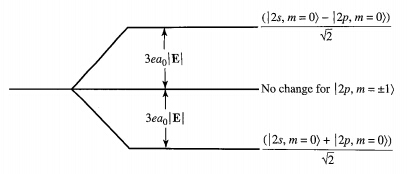
\includegraphics[width = 10cm]{./Graph/5.1.jpg}
\caption{一个作为简并微扰理论范例的线性斯塔克效应能级示意图}
\label {Figure 5.1}
\end{centering}
\end{figure}

现在我们可以问一个有趣的问题了。如果我们来看“实际的”氢原子,$2s$能级与$2p$能级并没有真的简并。由于自旋轨道力,$2p_{3/2}$ 会从$2p_{1/2}$ 能级被分开,正如我们将在下一节展示的,而且即便是遗留在单粒子狄拉克理论中的$2s_{1/2}$ 和$2p_{1/2}$间的简并度也会被量子电动力学效应(\emph{兰姆位移})移除。 我们可能因此问到,用简并微扰理论处理这个问题现实吗?一个与严格结果的对比体现出如果微扰矩阵元在与兰姆位移劈裂相比时大得多,那么在实用目的下看能移关于$|\boldsymbol{E}|$是线性的并且简并微扰理论的公式也是可用的。 在相反的极限下,假如微扰矩阵元在与兰姆位移劈裂相比时较小,那么能移就是二次的而且我们可以运用非简并微扰理论;见本章问题13。 这恰好体现出当能级与微扰矩阵元定义的能标相比几乎简并时简并微扰理论的方法依旧是有效的。对于两者之间的问题我们则需要一些更复杂的工作;尝试在临近能级生成的空间下将哈密顿量完全对角化是一个很保险的方法。

\subsection{类氢原子:精细结构与塞曼效应}

\

\noindent \textbf{动能的相对论修正}

\noindent 一个具有单电子的类氢原子有势能函数(\ref{3.7.43}),给出哈密顿量为

\begin{equation} \label{5.3.1}
H_0 = \dfrac{\boldsymbol{p}^2}{2m_e}-\dfrac{Ze^2}{r}\text{,}
\end{equation}

\noindent 其中第一项是非相对论性动能算符。然而,相对论修正后动能为

\begin{equation} \label{5.3.2}
K=\sqrt{\boldsymbol{p}^2c^+m_e^2c^4}-m_ec^2\approx \dfrac{\boldsymbol{p}^2}{2m_e}-\dfrac{(\boldsymbol{p}^2)^2}{8m_e^3c^2}\text{。}
\end{equation}

\noindent 因此,效仿(\ref{5.1.1})中的表示,我们可以用微扰理论处理这个问题,其中(\ref{5.3.1})给出$H_0$而微扰即是

\begin{equation} \label{5.3.3}
V= -\dfrac{(\boldsymbol{p}^2)^2}{8m_e^3c^2}\text{。}
\end{equation}

原则上来看,由于氢原子本征态$|nlm\rangle$具有极高简并度所以这是一个很复杂的问题。然而由于$\boldsymbol{L}$ 与$\boldsymbol{p}^2$对易,正如我们在(\ref{3.7.2}) 中所示,我们还有

\begin{equation} \label{5.3.4}
[\boldsymbol{L},V]=0\text{。}
\end{equation}

\noindent 换句话说,$V$是旋转对称的所以它在$|nlm\rangle$基下已经对角化了。因此,$V$ 产生的一阶能移就等于在这组基底态中的期望值。根据(\ref{5.1.37}),我们有

\begin{equation} \label{5.3.5}
\Delta_{nl}^{(1)}=\langle nlm|V|nlm\rangle = -\langle nlm|\dfrac{(\boldsymbol{p}^2)^2}{8m_e^3c^2}|nlm\rangle\text{,}
\end{equation}

\noindent 此处的旋转对称性保证了一阶能移不可能依赖于$m$。

原则上,(\ref{5.3.5})可以被暴力求解,但是这里有一种更优雅的方式。因为

\begin{equation} \label{5.3.6}
\dfrac{(\boldsymbol{p}^2)^2}{8m_e^3c^2}=\dfrac{1}{2m_ec^2} \left(\dfrac{\boldsymbol{p}^2}{2m_e}\right)^2 =\dfrac{1}{2m_ec^2}\left(H_0+\dfrac{Ze^2}{r}\right)^2\text{,}
\end{equation}

\noindent 我们立即看出

\begin{equation} \label{5.3.7}
\Delta_{nl}^{(1)}=-\dfrac{1}{2m_ec^2}\left[\left(E_n^{(0)}\right)^2+2E_n^{(0)}\langle nlm|\dfrac{Ze^2}{r}|nlm\rangle+\langle nlm|\dfrac{(Ze^2)^2}{r^2}|nlm\rangle\right]\text{。}
\end{equation}

\noindent 这个问题便退化成计算$Ze^2/r$与$(Ze^2)^2/r^2$ 的期望值。事实上,这两个期望值都可以用一些技巧来求解。我们在此只介绍一下手段,有兴趣的读者可以参考Shankar(1994) 或Townsend(2000) 来了解更多细节。

假如想象氢原子受到一个“扰动”$V_\gamma=\gamma/r$,那么(\ref{5.3.7})中第二项的期望值就只是$\gamma=Ze^2$ 时的一阶能量修正。另一方面,严格求解这个问题很简单,因为它对应着$Ze^2\rightarrow Ze^2-\gamma$的氢原子,而且由严格解可以直接找到一阶修正。可以发现

\begin{equation} \label{5.3.8}
\langle nlm|\dfrac{Ze^2}{r}|nlm\rangle = -2E_n^{(0)}\text{。}
\end{equation}

\noindent 其实,这实际上就是位力定理针对库伦势的一个结论。

我们也可以对(\ref{5.3.7})中第三项使用相同的手段。这种情况下,想象一个扰动$V_\gamma=\gamma/r^2$调整了有效势中的离心势垒项。也就是将$l$ 变为一个包含$\gamma$ 的形式,这样就可以用它写出一阶修正。我们发现

\begin{equation} \label{5.3.9}
\langle nlm|\dfrac{(Ze^2)^2}{r^2}|nlm\rangle = \dfrac{4n}{l+\frac{1}{2}}\left(E_n^{(0)}\right)^2\text{。}
\end{equation}

相应的,通过运用(\ref{5.3.8})和(\ref{5.3.9})以及(\ref{3.7.53})中的$E_n^{(0)}$,我们将(\ref{5.3.7}) 重写为

\begin{subequations}
\begin{align} \label{5.3.10}
\Delta_{nl}^{(1)}&=E_n^{(0)}\left[\dfrac{Z^2\alpha^2}{n^2}\left(- \dfrac{3}{4}+\dfrac{n}{l+\frac{1}{2}}\right)\right]\\
&=-\dfrac{1}{2}m_ec^2Z^4\alpha^4\left[- \dfrac{3}{4n^4}+\dfrac{1}{n^3\left(l+\frac{1}{2}\right)}\right]\text{。}
\end{align}
\end{subequations}

\noindent 不出所料,一阶修正的相关大小与$Z^2\alpha^2$成正比,即经典电子轨道速度的平方(单位为$c$)。

\noindent \textbf{自旋-轨道相互作用与精细结构}

\noindent 现在我们来学习一般类氢原子的原子能级,即,满壳层外只有一个价电子的原子。碱金属原子如钠(Na)和钾原子(K)都属于这种原子。

价电子受到的中心势(不依赖自旋)$V_c(r)$不再是纯库伦势形式。这是因为出现在

\begin{equation} \label{5.3.11}
V_c(r)=e\phi(r)
\end{equation}

\noindent 中的静电势$\phi{r}$不再只由原子核电量$|e|Z$决定;我们需要计入内壳中的负电荷云。此处我们不关心$\phi(r)$ 的精确形式。我们只需要提到纯库伦势的简并度特征因为给对于定$n$的高$l$态变得更高而消除了。物理上,这是由于$l$ 更高的态对于电子云产生的排斥表现的更敏感。

我们不必要学习这个决定了类氢原子糟糕结构的$V_c(r)$,反而来讨论这一导致\emph{精细结构}的自旋- 轨道相互作用$({\boldsymbol{L\cdot S}})$ 的效果。我们可以通过定量方式来理解这个相互作用的存在。由于中心力部分(\ref{5.3.11}),价电子会遭受电场

\begin{equation} \label{5.3.12}
{\boldsymbol{E}}=-\left(\dfrac{1}{e}\right)\nabla V_c(r)\text{。}
\end{equation}

\noindent 但是只要移动电荷被置入电场,它就会“感受到”一个有效磁场为

\begin{equation} \label{5.3.13}
{\boldsymbol{B}}_{e\!f\!f}=-\left(\dfrac{{v}}{c}\right)\times {\boldsymbol{E}}\text{。}
\end{equation}

\noindent 由于电子有一个磁矩$\boldsymbol{\mu}$为

\begin{equation} \label{5.3.14}
{\boldsymbol{\mu}}=\dfrac{e\boldsymbol{S}}{m_e c}\text{,}
\end{equation}

\noindent 我们因此猜测一个自旋轨道势$V_{LS}$对$H$的贡献如下:

\begin{equation} \label{5.3.15}
\begin{split}
H_{LS}\overset{?}{=}&-{\boldsymbol{\mu\cdot B}_{e\!f\!f}} \\
=&{\boldsymbol{\mu\cdot}}\left(\dfrac{\boldsymbol{v}}{c}\times {\boldsymbol{E}}\right) \\
=&\left(\dfrac{e\boldsymbol{S}}{m_ec}\right)\boldsymbol{\cdot} \left[\dfrac{\boldsymbol{p}}{m_e c}\times \left(\dfrac{\boldsymbol{x}}{r}\right)\dfrac{1}{(-e)}\dfrac{dV_c}{dr}\right] \\
=&\dfrac{1}{m_e^2c^2}\dfrac{1}{r}\dfrac{dV_c}{dr}({\boldsymbol{L\cdot S}})\text{。}
\end{split}
\end{equation}

\noindent 当这一表示与观测到的自旋轨道相互作用进行对比时,可以看出来它有正确的符号,但是数量却由于因子2而变得太大了。这里有一个引入自旋进动(以L.H.Thomas命名的\emph{托马斯进动})的经典解释,但是我们没必要考虑它。参见Jackson(1975)。 我们仅仅唯象地处理自旋轨道相互作用并取$V_{LS}$ 为(\ref{5.3.15}) 的一半。这一偏差的正确量子力学解释需要等到本书最后一章对电子的狄拉克(相对论性)理论的讨论。

我们现在就需要取$V_{LS}$为扰动(5.1和5.2节中的$V$)来对氢原子运用微扰理论。非微扰哈密顿量$H_0$ 写作

\begin{equation} \label{5.3.16}
H_0=\dfrac{\boldsymbol{p}^2}{2m}+V_c(r)\text{,}
\end{equation}

\noindent 其中的中心势$V_c$不再是碱金属的纯库伦势形式。在有$H_0$后,我们便有了选择基矢的自由:

\begin{equation} \label{5.3.17}
\begin{split}
\text{集合 1:}{\boldsymbol{L}}^2,L_z,{\boldsymbol{S}}^2,S_z\text{的本征右矢。} \\
\text{集合 2:}{\boldsymbol{L}}^2,{\boldsymbol{S}}^2,{\boldsymbol{J}}^2,J_z\text{的本征右矢。}
\end{split}
\end{equation}

\noindent 不考虑$V_{LS}$(或$H_{LS}$)时在基矢也是能量本征右矢的意义下两个集合都是合理的。考虑$H_{LS}$后,使用(\ref{5.3.17})中的集合2便有了很大的优越性因为$\boldsymbol{L\cdot S}$与$L_z$和$S_z$不对易,但是与$\boldsymbol{J}^2$和$J_z$对易。 记住最基本的要求:选择可以将扰动对角化的非微扰右矢。如果你用$L_z$ 和$S_Z $ 的本征右矢[(\ref{5.3.17}) 中的集合1] 作为这个问题的基矢那么你不是傻瓜就是受虐狂;如果在选用集合1位我们的基矢后盲目的运用简并微扰理论的方法,那么我们就不得不在$L_z$,$S_z$表示下将$V_{LS}$($H_{LS}$)矩阵对角化。这种方法的结果,在经历繁杂的代数运算后,将会给出与取$\boldsymbol{J}^2$,$J_z$本征右矢为零阶非微扰右矢后一样的结果!

在简并微扰理论中,如果在我们选取的表示下微扰以及是对角化的,那么我们想要一阶能移便只需要求期望值。波函数的二分量形式可以明确表示为

\begin{equation} \label{5.3.18}
\psi_{nlm}=R_{nl}(r)\mathcal{Y}_l^{j=l\pm 1/2,m}\text{,}
\end{equation}

\noindent 其中$\mathcal{Y}_l^{j=l\pm1/2,m}$是3.8节的自旋角函数[见(\ref{3.8.64})]。对于一阶能移,我们得到

\begin{equation} \label{5.3.19}
\begin{split}
\Delta_{nlj}&=\dfrac{1}{2m_e^2c^2}\left\langle\dfrac{1}{r}\dfrac{dV_c}{dr}\right\rangle_{nl} \dfrac{\hbar^2}{2}\left\{\begin{array}{c}
l \\
-(l+1)
\end{array}\right\}\begin{array}{c}
j=l+\frac{1}{2} \\
j=l-\frac{1}{2}
\end{array} \\
\left\langle\dfrac{1}{r}\dfrac{dV_c}{dr}\right\rangle_{nl}&\equiv \displaystyle\int_0^{\infty}R_{nl}\dfrac{1}{r}\dfrac{dV_c}{dr}R_{nl}r^2dr\text{,}
\end{split}
\end{equation}

\noindent 其中我们运用了独立于$m$的恒等式[见(\ref{3.8.66})]。

\begin{equation} \label{5.3.20}
\displaystyle\int \mathcal{Y}^{\dag} \boldsymbol{S\cdot L}\mathcal{Y}d\Omega= \dfrac{1}{2}\left[j(j+1)-l(l+1)-\dfrac{3}{4}\right]\hbar^2 =\dfrac{\hbar^2}{2}\left\{\begin{array}{c}
l \\
-(l+1)\end{array}\right\}\begin{array}{c}
j=l+\frac{1}{2} \\
j=l-\frac{1}{2} \end{array}\text{。}
\end{equation}

\noindent 方程(\ref{5.3.19})叫做{\textbf{朗德间隔定则}}。

更细致的来说,考虑一个钠原子。由标准原子光谱学记号可知,基态的结构为

\begin{equation} \label{5.3.21}
(1s)^2(2s)^2(2p)^6(3s)\text{。}
\end{equation}

\noindent 壳内的10个电子可以被视作组成一个球对称性电子云。我们对于第11个电子由$3s$向更高态的激发过程感兴趣。最近的可能情况是到$3p$的激发。由于中心势不再是纯库伦势形式,$3s$ 与$3p$能级现在被劈裂。$V_{LS}$ 所导致的精细结构甚至依赖于$3p$中更精细的劈裂,其位于$3p_{1/2}$与$3p_3/2$间,其中的角标依赖于$j$。实验上,我们观测到两个近距离分离的黄色谱线,即钠的$D$ 谱线,一个位于$5,896\overset{\circ}{A}$ ,另一个位于$5,890\overset{\circ}{A}$;见图{\ref{Figure 5.2}}。 注意到$3p_{3/2}$ 的位置要更高一些这是因为(\ref{5.3.19}) 中径向积分是正的。

\begin{figure}
\begin{centering}
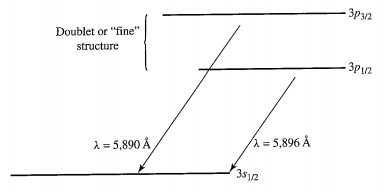
\includegraphics[width = 10cm]{./Graph/5.2.jpg}
\caption{$3s$与$3p$谱线的示意图。$3s$与$3p$的简并度被提升因为$V_c(r)$现在是核心电子导致的屏蔽库伦势而非纯库伦势;$V_{LS}$也移除了$3p_{1/2}$与$3p_{3/2}$的简并度。}
\label {Figure 5.2}
\end{centering}
\end{figure}


为了更好地体会到精细结构劈裂的数量级,我们注意到对于$Z\simeq 1$,

\begin{equation} \label{5.3.22}
\left\langle\dfrac{1}{r}\dfrac{dV_c}{dr}\right\rangle_{nl}\sim\dfrac{e^2}{a_0^3}
\end{equation}

\noindent 恰好符合量纲的考虑。因此精细结构劈裂的数量级为$(e^2/a_0^3)(\hbar/m_ec)^2$,其与巴尔末劈裂的数量级$e^2/a_0$形成对比。 值得一提的是经典电子半径,电子的康普顿波长,和玻尔半径间的关系如下:

\begin{equation} \label{5.3.23}
\dfrac{e^2}{m_ec^2}:\dfrac{\hbar}{m_ec}:a_0::1:137:(137)^2\text{,}
\end{equation}

\noindent 其中我们用到

\begin{equation} \label{5.3.24}
\dfrac{e^2}{\hbar c}=\dfrac{1}{137}\text{。}
\end{equation}

\noindent 很特殊地,精细结构劈裂与经典巴尔末劈裂的关系为

\begin{equation}
\left(\dfrac{e^2}{a_0^3}\dfrac{\hbar^2}{m_e^2 c^2}\right):\left(\dfrac{e^2}{a_0}\right) ::\left(\dfrac{1}{137}\right)^2:1\text{,}
\end{equation}

\noindent 这便解释了精细结构项的来源。还有其他一些效应有着相同的数量级;一个例子就是在之前小节里讨论的动能的相对论性修正。

在结束这一讨论前,我们来算出库伦势问题下的(\ref{5.3.19}),即,氢原子或拥有$Z$ 个质子的单电子离子。这种情况下

\begin{equation} \label{5.3.26}
\left\langle\dfrac{1}{r}\dfrac{dV_c}{dr}\right\rangle_{nl}= \left\langle\dfrac{Ze^2}{r^3}\right\rangle_{nl}\text{。}
\end{equation}

\noindent 我们还需要另一种技巧来求解这个期望值。首先我们注意到根据(\ref{5.3.1})所给出的$H_0$,我们有

\begin{equation} \label{5.3.27}
\langle nlm|[H_0,A]|nlm\rangle=0
\end{equation}

\noindent 对于\emph{任意}算符$A$成立,因为$H_0$作用在右边或左边只给出$E_n^{(0)}$。如果我们令$A=p_r$,即径向动量算符,那么它很明显与$H_0$中动能项的径向部分对易。因此,我们便有

\begin{equation} \label{5.3.28}
\langle nlm|\left[\dfrac{l(l+1)\hbar^2}{2m_er^2}-\dfrac{Ze^2}{r},p_r\right]|nlm\rangle=0\text{。}
\end{equation}

\noindent 现在在坐标空间中,$p_r$与坐标$r$的函数不对易因为倒数$\partial/\partial r$存在。因此,我们可以明显由(\ref{5.3.28}) 中的交换子得到

\begin{equation} \label{5.3.29}
\langle nlm|\left[-\dfrac{l(l+1)\hbar^2}{m_er^3}+\dfrac{Ze^2}{r^2}\right]|nlm\rangle=0\text{。}
\end{equation}

\noindent 最后,我们通过(\ref{5.3.9})与(\ref{3.7.53})得出

\begin{equation} \label{5.3.30}
\begin{split}
\left\langle\dfrac{Ze^2}{r^3}\right\rangle_{nl} &=\dfrac{m_e}{l(l+1)\hbar^2}\left\langle\dfrac{(Ze^2)^2}{r^2}\right\rangle_{nl} \\
&=-\dfrac{2m_e^2c^2Z^2\alpha^2}{nl(l+1)(l+1/2)\hbar^2}E_n^{(0)}\text{。}
\end{split}
\end{equation}

\noindent  我们因此从(\ref{5.3.19})得到了氢原子能量本征态的自旋轨道修正为

\begin{equation} \label{5.3.31}
\Delta_{nlj}=-\dfrac{Z^2\alpha^2}{2nl(l+1)(l+1/2)}E_n^{(0)}\left\{\begin{array}{c}
l \\
-(l+1)
\end{array}\right\}\begin{array}{c}
j=l+\frac{1}{2} \\
j=l-\frac{1}{2}
\end{array}\text{。}
\end{equation}

\noindent 很有趣的是,当$l=0$时这个表达式是非零的。不过,它却给出了狄拉克方程能量本征值的正确答案,正如本书后面将要看到的。这个能移的起因,归结于一个Darwin 项,在别处有所讨论。比如可以阅读Townsend(2000)。

\noindent \textbf{塞曼效应}

\noindent 现在我们来讨论氢原子或类氢(单电子)原子在固定磁场的情况,即塞曼效应,有时在考虑电子自旋后被叫做反常塞曼效应。重新提到固定磁场$B$ 可由矢势

\begin{equation} \label{5.3.32}
\boldsymbol{A}=\frac{1}{2}(\boldsymbol{B}\times\boldsymbol{r})
\end{equation}

\noindent 导出。对于$z$轴正方向的$\boldsymbol{B}$($\boldsymbol{B}=B\boldsymbol{\hat{z}}$),既是

\begin{equation} \label{5.3.33}
\boldsymbol{A}=-\frac{1}{2}(By\boldsymbol{\hat{x}}-Bx\boldsymbol{\hat{y}})
\end{equation}

\noindent 其中$B$代表$|\boldsymbol{B}|$。抛弃自旋项,相互作用哈密顿量由代换

\begin{equation} \label{5.3.34}
\boldsymbol{p}\rightarrow\boldsymbol{p}-\dfrac{e\boldsymbol{A}}{c}
\end{equation}

\noindent 生成。我们因此有

\begin{equation} \label{5.3.35}
H=\dfrac{\boldsymbol{p}^2}{2m_e}+V_c(r)-\dfrac{e}{2m_ec} (\boldsymbol{p\cdot A}+\boldsymbol{A\cdot p})+\dfrac{e^2\boldsymbol{A}^2}{2m_ec^2}
\end{equation}

\noindent 由于

\begin{equation} \label{5.3.36}
\langle\boldsymbol{x}'|\boldsymbol{p\cdot A}(\boldsymbol{x})|\rangle=-i\hbar\boldsymbol{\nabla}'\boldsymbol{\cdot}[\boldsymbol{A} (\boldsymbol{x}')\langle\boldsymbol{x}'|\rangle])=\langle\boldsymbol{x}'|\boldsymbol{A}(\boldsymbol{x})\boldsymbol{ \cdot p}|\rangle+\langle\boldsymbol{x}'|\rangle[-i\hbar\boldsymbol{\nabla}'\boldsymbol{\cdot A}(\boldsymbol{x}')]\text{,}
\end{equation}

\noindent 只要满足

\begin{equation} \label{5.3.37}
\boldsymbol{\nabla\cdot A}(\boldsymbol{x})=0
\end{equation}

\noindent 就可以合理地替换$\boldsymbol{p\cdot A}$为$\boldsymbol{A\cdot p}$,这也是(\ref{5.3.33})中的矢势所满足的。注意到

\begin{equation} \label{5.3.38}
\begin{split}
\boldsymbol{A\cdot p}&=|\boldsymbol{B}|(-\frac{1}{2}yp_x+\frac{1}{2}xp_y) \\
&=\frac{1}{2}|\boldsymbol{B}|L_z
\end{split}
\end{equation}

\noindent 且

\begin{equation} \label{5.3.39}
\boldsymbol{A}^2=\frac{1}{4}|\boldsymbol{B}|^2(x^2+y^2)\text{,}
\end{equation}

\noindent 我们从(\ref{5.3.35})得到

\begin{equation} \label{5.3.40}
H=\dfrac{\boldsymbol{p}^2}{2m_e}+V_c(r)-\dfrac{e}{2m_ec}|\boldsymbol{B}|L_z+ \dfrac{e^2}{8m_ec^2}|\boldsymbol{B}|^2(x^2+y^2)\text{。}
\end{equation}

\noindent 由此我们便可以考虑自旋磁矩相互作用

\begin{equation} \label{5.3.41}
-\boldsymbol{\mu\cdot B}=\dfrac{-e}{m_ec}\boldsymbol{S\cdot B}=\dfrac{-e}{m_ec}|\boldsymbol{B}|S_z\text{。}
\end{equation}

\noindent 二次项$|\boldsymbol{B}|^2(x^2+y^2)$对于单电子原子来说并不重要;类似的项对于$L_z^{(tot)}$ 与$S_z^{(tot)}$ 均为零的氦原子基态很重要。读者可以在本章习题5.18 和5.19 中计算抗磁磁化率后再回来考虑这个问题。

总而言之,省略二次项后,总哈密顿量就只由下列三项组成的:

\begin{subequations} \label{5.3.42a}
\begin{align}
H_0&=\dfrac{\boldsymbol{p}^2}{2m_e}+V_c(r)\\
 \label{5.3.42b}
H_{LS}&=\dfrac{1}{2m_e^2c^2r}\dfrac{1}{r}\dfrac{dV_c(r)}{dr}\boldsymbol{L\cdot S}\\
\label{5.3.42c}
H_B&=\dfrac{-e|\boldsymbol{B}|}{2m_ec}(L_z+2S_z)\text{。}
\end{align}
\end{subequations}

\noindent 注意到$S_z$前的系数2;这反映了电子的$g$因子是2这一事实。

假设将$H_B$看做一个很小的扰动。我们可以通过将$H_0+H_{LS}$的本征右矢,即$\boldsymbol{J}^2$,$J_z$的本征右矢,作为基矢来学习$H_B$的作用。注意到

\begin{equation} \label{5.3.43}
L_z+2S_z=J_z+S_z\text{,}
\end{equation}

\noindent 因此我们可以将一阶能移写为

\begin{equation} \label{5.3.44}
\dfrac{-e|\boldsymbol{B}|}{2e_mc}\langle J_z+S_z\rangle_{j=l\pm 1/2,m}\text{。}
\end{equation}

\noindent $J_z$的期望值易得为$m\hbar$。至于$\langle S_z\rangle$,我们首先重提

\begin{equation} \label{5.3.45}
\begin{split}
\left|j=l\pm\dfrac{1}{2},m\right\rangle=&\pm\sqrt{\dfrac{l\pm m+\frac{1}{2}}{2l+1}}\left|m_l=m-\dfrac{1}{2},m_s=\dfrac{1}{2}\right\rangle \\
& +\sqrt{\dfrac{l\mp m+\frac{1}{2}}{2l+1}}\left|m_l=m+\dfrac{1}{2},m_s=-\dfrac{1}{2}\right\rangle\text{。}
\end{split}
\end{equation}

\noindent $S_z$的期望值可以轻松求得:

\begin{equation} \label{5.3.46}
\begin{split}
\langle S_Z\rangle_{j=l\pm 1/2,m}&=\dfrac{\hbar}{2}(|c_+|^2-|c_-|^2) \\
&=\dfrac{\hbar}{2}\dfrac{1}{(2l+1)}\left[\left(l\pm m+\dfrac{1}{2}\right)-\left(l\mp m+\dfrac{1}{2}\right)\right] \\
&=\pm \dfrac{m\hbar}{(2l+1)}\text{。}
\end{split}
\end{equation}

\noindent 通过这种方法我们得到了($\boldsymbol{B}$场导致的)能移的朗德公式

\begin{equation} \label{5.3.47}
\Delta E_B=\dfrac{-e\hbar B}{2m_ec}m\left[1\pm\dfrac{1}{(2l+1)}\right]\text{。}
\end{equation}

我们看到(\ref{5.3.47})中的能移与$m$成比例。为了理解其中的物理解释,我们来展示另一种导出(\ref{5.3.46})的方法。我们重提$S_z$的期望值可以用3.11节提到的射影定理来取得。我们得到[见(\ref{3.11.45})]

\begin{equation} \label{5.3.48}
\begin{split}
\langle S_z\rangle_{j=l\pm 1/2,m}&=\left[\langle\boldsymbol{S\cdot J}\rangle_{j=l\pm 1/2}\right]\dfrac{m\hbar}{\hbar^2j(j+1)} \\
&= \dfrac{m\langle\boldsymbol{J}^2 +\boldsymbol{S}^2-\boldsymbol{L}^2\rangle_{j=l\pm 1/2}}{2\hbar j(j+1)} \\
&= m\hbar\left[\dfrac{\left(l\pm\frac{1}{2}\right)\left(l\pm\frac{1}{2}+1\right)+ \frac{3}{4}-l(l+1)}{2\left(l\pm \frac{1}{2}\right)\left(l\pm \frac{1}{2}+1\right)}\right] \\
&=\pm\dfrac{m\hbar}{(2l+1)}\text{,}
\end{split}
\end{equation}

\noindent 其结果与(\ref{5.3.46})完全一致。

在先前的讨论中磁场都被看做一个微扰。我们现在来考虑极端相反情况,叫做Paschen-Back极限,即磁场的影响太剧烈以至于$H_B$的作用远重要于$H_{LS}$的作用,后者我们在接下来当做微扰来代入。在只有$H_0+H_B$时,好量子数为$L_z$和$S_z$。 即便$\boldsymbol{J}^2$ 也不够好因为球对称性被特定方向,即$z$方向,的强$\boldsymbol{B}$场完全破坏了。我们便只剩下柱对称性了,即,绕$z$ 轴旋转不变性。因此$L_z$,$S_z$的本征右矢$|l,s=\frac{1}{2},m_l,m_s\rangle$就要被作为我们的基矢了。主项$H_B$的影响可以很快计算出来:

\begin{equation} \label{5.3.49}
\langle H_B\rangle_{m_lm_s}=\dfrac{-e|\boldsymbol{B}|\hbar}{2m_ec}(m_l+2m_s)\text{。}
\end{equation}

\noindent $H_0$[见(\ref{5.3.42a})]中原有的在$m_l$和$m_s$中的$2(2l+1)$重简并度现在被$H_B$缩减来保持相同的$(m_l)+(2m_s)$,也就是,$(m_l)+(1)$和$(m_l+2)+(-1)$。 很明显我们需要计算$\boldsymbol{L\cdot S}$依赖于$|m_l,m_s\rangle$的期望值:

\begin{equation} \label{5.3.50}
\begin{split}
\langle\boldsymbol{L\cdot S}\rangle&= \langle L_zS_z+\frac{1}{2}(L_+S_-+L_-S_+)\rangle_{m_lm_s} \\
&=\hbar^2m_lm_s\text{,}
\end{split}
\end{equation}

\noindent 其中我们用到了

\begin{equation} \label{5.3.51}
\langle L_\pm\rangle_{m_l}=0,\quad\langle S_\pm\rangle_{m_s}=0\text{。}
\end{equation}

\noindent 因此,

\begin{equation} \label{5.3.52}
\langle H_{LS}\rangle_{m_lm_s}=\dfrac{\hbar^2m_lm_s}{2m_e^2c^2} \left\langle\dfrac{1}{r}\dfrac{dV_c}{dr}\right\rangle\text{。}
\end{equation}

在很多的基础书里都会有关于弱磁场(\ref{5.3.47})和强磁场(\ref{5.3.49})的列表解读,但是我们在此不讨论他们。

\begin{centering}
\begin{table}[!hbp]
\begin{tabular}{p{1.7cm}p{2.4cm}p{2.4cm}c|p{2.4cm}}
\hline
 & \textbf{主要相互作用}& \textbf{几乎好量子数}& \textbf{不是好量子数} & \textbf{总是好量子数}\\
\hline
弱磁场$\bm B$ & $H_{LS}$ & $\bm{J^2} \text{(或} \bm{L\cdot S}\text{)}$ & $L_z,\ S_z$ \\
强磁场$\bm B$ & $H_B$ & $L_z,\ S_z$ & $\bm{J^2} \text{(或} \bm{L\cdot S}\text{)}$ & \raisebox{2ex}[0pt]{$\bm{L^2,\ S^2},\ S_z$} \\
\hline
\end{tabular}
\caption{表格5.1}
\end{table}
\end{centering}

\noindent 我们简短的来总结一下表格5.1的结果,其中强场和弱场的“划分”以他们的数量级$e\hbar B/2m_ec$ 与$(1/137)^2e^2/a_0$对比而得。表格中的\emph{几乎好量子数}是在次要相互作用几乎可以被忽略时才是好的。

尤其地,我们来看一个$p$电子$l=1(p_{3/2},p_{1/2}$的能级图。在弱$\boldsymbol{B}$情况下,能移与$\boldsymbol{B}$ 是线性的,其斜率由

\begin{equation}
m\left[1\pm\left(\dfrac{1}{2l+1}\right)\right]
\end{equation}

\noindent 决定。随着我们增高$\boldsymbol{B}$,具有相同$m$的态之间的混合变得更有可能,比如,$m=\pm\frac{1}{2}$ 的$p_{3/2}$与$m=\pm\frac{1}{2}$的$p_{1/2}$;在这种关联下注意到在$H_B$中出现的算符$L_z+2S_z$是一个一阶张量算符$T_{q=0}^{(k=1)}$且球面分量$q=0$。 在夹在中间的$\boldsymbol{B}$ 的情况下,仅用如(\ref{5.3.47}) 与(\ref{5.3.49}) 的公式计算期望值是不可能的;我们需要去将对应的$2\times2$ 矩阵对角化(Gotfried and Yan 2003, Section 5.4)。在强$\boldsymbol{B}$极限下,能移再次与$|\boldsymbol{B}|$ 成比例;如同我们在(\ref{5.3.49}) 中看到的,斜率由$m_l+2m_s$决定。

\noindent \textbf{范德瓦尔斯相互作用}

\noindent 一个很重要,而且很好的瑞利-薛定谔微扰理论的应用就是计算两个位于他们基态的氢原子间的长程相互作用,或{\textbf{范德瓦尔斯力}}。我们很容易得出两个距离$r$很远的原子间的能量是吸引的且以$r^{-6}$变化。

考虑两个氢原子的质子(沿$z$轴)\emph{固定}距离为$r$且$\boldsymbol{r}_1$是第一个质子到其电子的位矢而$\boldsymbol{r}_2$是第二个质子到其电子的位矢;见图5.3。 则哈密顿量$H$ 可以被写作

\begin{equation} \label{5.3.53}
\begin{split}
H &=H_0+V \\
H_0 &=-\dfrac{\hbar^2}{2m}(\nabla_1^2+\nabla_2^2)-\dfrac{e^2}{r_1}-\dfrac{e^2}{r_2} \\
V &=\dfrac{e^2}{r}+\dfrac{e^2}{|\boldsymbol{r}+\boldsymbol{r}_2-\boldsymbol{r}_1|} -\dfrac{e^2}{|\boldsymbol{r}+\boldsymbol{r}_2|}- \dfrac{e^2}{|\boldsymbol{r}-\boldsymbol{r}_1|}\text{。}
\end{split}
\end{equation}

\begin{figure}
\begin{centering}
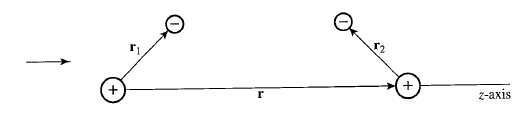
\includegraphics[width = 10cm]{./Graph/5.3.jpg}
\caption{两个氢原子及它们的质子(+)相聚固定的距离$r$且他们的电子(-)相对位矢为$\boldsymbol{r}_i$。}
\label {Figure 5.3}
\end{centering}
\end{figure}

\

\noindent $H_0$的最低能量解就仅是不进行相互作用的氢原子基态波函数之积

\begin{equation} \label{5.3.54}
U_0^{(0)}=U_{100}^{(0)}(\boldsymbol{r}_1)U_{100}^{(0)}(\boldsymbol{r}_2)\text{。}
\end{equation}

\noindent 那么对于极大的$r$($\gg$玻尔半径$a_0$),将扰动$V$展开为$\boldsymbol{r}_i/\boldsymbol{r}$的幂便可以得到

\begin{equation} \label{5.3.55}
V=\dfrac{e^2}{r^3}(x_1x_2+y_1y_2-2z_1z_2)+O\left(\dfrac{1}{r^4}\right)+\cdots\text{。}
\end{equation}

\noindent (\ref{5.3.55})中的最低阶$r^{-3}$项对应于相距$\boldsymbol{r}$的两个电偶极子$e\boldsymbol{r}_1$ 与$e\boldsymbol{r}_2$间的相互作用。更高阶项代表着高阶多极子相互作用,而且因此$V$中每一项都包含球谐函数$Y_l^m$其中对于每个氢原子有$l_i>0$。因此,对于(\ref{5.3.55})中的每一项其一阶微扰能量矩阵元$V_{00}\simeq0$,因为基态$U_0^{(0)}$波函数(\ref{5.3.54})有$l_i=0$以及对于$l$和$m\neq0$有$\int d\Omega Y_l^m(\Omega)=0$。二阶微扰

\begin{equation} \label{5.3.56}
E^{(2)}(r)=\dfrac{e^4}{r^6}\displaystyle\sum_{k\neq0}\dfrac{|\langle k^{(0)}|x_1x_2+y_1y_2-2z_1z_2| 0^{(0)}\rangle|^2}{E_0^{(0)}-E_k^{(0)}}
\end{equation}

\noindent 将会不会为零。我们很快可以看出这个相互作用随$1/r^6$变化;因为$E_0^{(0)}>E_k^{(0)}$,它是负的。这个$1/r^6$长程吸引范德瓦尔斯势是两个处于基态的原子普遍存在的相互作用性质。

\subsection{变分法}

\

\noindent 我们上一节所介绍的微扰理论,当然,除非我们已经知道一个哈密顿量足够相似的问题的严格解否则是没有用的。我们现在要讨论的变分法在没有这种严格解的情况下求解基态能量$E_0$是非常有效的。

\noindent 我们通过考虑一个“平凡右矢”$|\tilde{0}\rangle$来尝试猜测基态能量$E_0$,即尝试仿造出真实的基态右矢$|0\rangle$。以这个为目的我们首先得到一个具有极大应用价值的定理。我们定义$\bar{H}$为

\begin{equation} \label{5.4.1}
\bar{H}=\dfrac{\langle\tilde{0}|H|\tilde{0}\rangle}{\langle\tilde{0}|\tilde{0}\rangle}\text{,}
\end{equation}

\noindent 其中我们兼容了$|\tilde{0}\rangle$不能被归一化的可能性。我们便可以紧接着证明。


\noindent \textbf{定理 5.1.}

\begin{equation} \label{5.4.2}
\bar{H}\geq E_0\text{。}
\end{equation}

\noindent 这意味着我们可以通过考虑多种类型的$|\tilde{0}\rangle$来得到一个$E_0$的上界。其证明是非常直观的。

\noindent \textbf{证明.} 即便我们不知道哈密顿量$H$的能量本征右矢,我们可以假设$|\tilde{0}\rangle$可以被展开成

\begin{equation} \label{5.4.3}
|\tilde{0}\rangle=\displaystyle\sum_{k=0}^{\infty}|k\rangle\langle k|\tilde{0}\rangle\text{,}
\end{equation}

\noindent 其中$|k\rangle$是$H$的一个\emph{严格}能量本征右矢:

\begin{equation} \label{5.4.4}
H|k\rangle=E_k|k\rangle\text{。}
\end{equation}

\noindent 等式(\ref{5.4.2})可以在我们用$E_k=E_k-E_0+E_0$计算(\ref{5.4.1})中的$\bar{H}$来的出。我们有

\begin{subequations} \label{5.4.5a}
\begin{align}
\bar{H}&=\dfrac{\displaystyle\sum_{k=0}|\langle k|\tilde{0}\rangle|^2E_k}{\displaystyle\sum_{k=0}|\langle k|\tilde{0}\rangle|^2}\\
\label{5.4.5b}
&=\dfrac{\displaystyle\sum_{k=1}^{\infty}|\langle k|\tilde{0}\rangle|^2(E_k-E_0)}{\displaystyle\sum_{k=0}|\ \langle k|\tilde{0}\rangle|^2}+E_0\\
\label{5.4.5c}
&\geq E_0\text{,}
\end{align}5
\end{subequations}

\noindent 其中我们用到了(\ref{5.4.5b})第一项中的$E_k-E_0$需要为正的事实。从这一证明也能很明显看出(\ref{5.4.2}) 中的符号仅当$|\tilde{0}\rangle$与$|0\rangle$恰好相同时才能成立,也就是,系数$\langle k|\tilde{0}\rangle$对于$k\neq 0$时都为零。

\noindent 定理(\ref{5.4.2})非常有效因为$\bar{H}$提供了一个实际基态能量的上界。而且,一个相关性很小的平凡右矢可以给出一个非常好的基态能量估值,因为如果

\begin{equation} \label{5.4.6}
\langle k|\tilde{0}\rangle\sim O(\varepsilon) \text{对于}k\neq0\text{,}
\end{equation}

\noindent 那么从(\ref{5.4.5})我们有

\begin{equation} \label{5.4.7}
\bar{H}-E_0\sim O(\varepsilon^2)\text{。}
\end{equation}

\noindent 我们将在接下来给出一个例子。当然,这一方法并没有说明$\bar{H}$与$E_0$间有哪些差异;我们唯一知道的就是$\bar{H}$要大于(或等于)$E_0$。

另一种阐述这一定理的方法是断言$\bar{H}$在变分

\begin{equation} \label{5.4.8}
|\tilde{0}\rangle\rightarrow|\tilde{0}\rangle+\delta|\tilde{0}\rangle
\end{equation}

\noindent 下是不变的;也就是,当$|\tilde{0}\rangle$恰好为$|0\rangle$时$\delta\bar{H}=0$。这样意味着如果用$|0\rangle+\delta|\tilde{0}\rangle$来替代(\ref{5.4.5a})中的$|\tilde{0}\rangle$并计算$\bar{H}$,那么我们在求实际基态能量时在$|\tilde{0}\rangle$中包含的误差是$(\delta|\tilde{0}\rangle)^2$阶的。

变分法本质上并没有告诉我们在估计基态能量时选取哪种类型的平凡右矢。一般来说我们需要求助于物理直觉,比如,在大距离下波函数的渐进行为。我们在实践中运用的方法是用一个或多个参数$\lambda_1,\lambda_2,\cdots$来刻画平凡右矢并把$\bar{H}$看做一个关于$\lambda_1,\lambda_2,\cdots$的函数来计算。我们紧接着最小化$\bar{H}$通过(1)令关于参数的倒数均为零,即

\begin{equation} \label{5.4.9}
\dfrac{\partial\bar{H}}{\partial\lambda_1}=0,\dfrac{\partial\bar{H}}{\partial\lambda_2}=0,\cdots\text{,}
\end{equation}

\noindent (2)确定$\lambda_1,\lambda_2,\cdots$的最优值,以及(3)将他们带回$\bar{H}$的表达式。

如果平凡右矢的波函数已经有了一个严格的基态能量本征函数的有效形式,我们当然通过这种方法得到了真实基态能量函数。比如说,假设某人有预见性地猜到了氢原子基态波函数需要有符合

\begin{equation} \label{5.4.10}
\langle\boldsymbol{x}|0\rangle\propto e^{-r/a}\text{,}
\end{equation}

\noindent 其中$a$被看做是一个可以调整的参数。我们接下来发现,在通过(\ref{5.4.10})将$\bar{H}$最小化后,能得到正确的基态能量$-e^2/2a_0$。不出意料,最小值可以在$a$恰为玻尔半径$a_0$时达到。

作为第二个例子,我们尝试求出定义为

\begin{equation} \label{5.4.11}
V=\begin{cases}
0, &|x|<a\\
\infty, &|x|>a
\end{cases}
\end{equation}

\noindent 的(一维)无限深方势阱问题的基态。问题的严格解,当然,我们知道是

\begin{equation} \label{5.4.12}
\begin{split}
\langle x|0\rangle&=\dfrac{1}{\sqrt{a}}\cos\left(\dfrac{\pi x}{2a}\right)\text{,}\\
E_0&=\left(\dfrac{\hbar^2}{2m}\right)\left(\dfrac{\pi^2}{4a^2}\right)\text{。}
\end{split}
\end{equation}

\noindent 但是假设我们不知道这些。很明显波函数必须在$x=\pm a$时为零;而且,对于基态其波函数不能有任何摆动。符合两个要求的最简单的解析函数就是通过$x=\pm a$的一个抛物线:

\begin{equation} \label{5.4.13}
\langle x|\tilde{0}\rangle=a^2-x^2
\end{equation}

\noindent 其中我们不去归一化$\tilde{0}\rangle$。这里没有变分参数。我们可以计算$\bar{H}$如下:

\begin{equation} \label{5.4.14}
\begin{split}
\bar{H}&=\dfrac{\left(\dfrac{-\hbar^2}{2m}\right)\displaystyle\int_{-a}^a(a^2-x^2)\dfrac{d^2}{dx^2}(a^2-x^2)dx} {\displaystyle\int_{-a}^a(a^2-x^2)dx}\\
&=\left(\dfrac{10}{\pi^2}\right)\left(\dfrac{\pi^2\hbar^2}{8a^2m}\right)\simeq1.0132E_0\text{。}
\end{split}
\end{equation}

\noindent 值得注意的是通过这样一个简单的平凡函数,我们可以得到的结果与实际基态能量偏差在$1.3\%$内。

如果我们用一个更复杂的平凡函数可以得到一个更好的结果。我们尝试

\begin{equation} \label{5.4.15}
\langle x|\tilde{0}\rangle=|a|^{\lambda}-|x|^{\lambda}\text{,}
\end{equation}

\noindent 其中$\lambda$现在被看做变分参数。通过代数过程直接得到

\begin{equation} \label{5.4.16}
\bar{H}=\left[\dfrac{(\lambda+1)(2\lambda+1)}{(2\lambda-1)}\right]\left(\dfrac{\hbar^2}{4ma^2}\right)\text{,}
\end{equation}

\noindent 它有一个极小值位于

\begin{equation} \label{5.4.1.7}
\lambda=\dfrac{1+\sqrt{6}}{2}\simeq1.72\text{,}
\end{equation}

\noindent 与先前考虑的$\lambda=2$(的抛物线)很接近。它给出

\begin{equation} \label{5.4.18}
\bar{H}_{min}=\left(\dfrac{5+2\sqrt{6}}{\pi^2}\right)E_0\simeq 1.00298E_0\text{。}
\end{equation}

\noindent 因此运用(\ref{5.4.15})的变分法给出的结果与正确基态能量偏差在$0.3\%$内,仅用简洁的平凡函数便给出了完美的答案。

那么这个平凡函数与真实的基态波函数到底有多吻合呢?令人愉悦的是回答这个问题并不用我们明确的求解重迭积分$\langle0|\tilde{0}\rangle$。假如$|\tilde{0}\rangle$已经归一化,我们[从(\ref{5.4.1})-(\ref{5.4.4})]有

\begin{equation} \label{5.4.19}
\begin{split}
\bar{H}_{min}&=\displaystyle\sum_{k=0}^{\infty}|\langle k|\tilde{0}\rangle|^2E_k\\
&\geq|\langle0|\tilde{0}\rangle|^2E_0+9E_0(1-|\langle0|\tilde{0}\rangle|^2)\text{,}
\end{split}
\end{equation}

\noindent 其中$9E_0$是第二激发态的能量;第一激发态($k=1$)由于宇称守恒而没有贡献。为了求解$|\langle0|\tilde{0}\rangle|$通过(\ref{5.4.18}),我们有

\begin{equation} \label{5.4.20}
|\langle0|\tilde{0}\rangle|^2\geq\dfrac{9E_0-\bar{H}_{min}}{8E_0}=0.99963\text{。}
\end{equation}

\noindent 与一的差异意味着$|\tilde{0}\rangle$的一个分量方向正交于$|0\rangle$。如果我们是讨论

\begin{equation} \label{5.4.21}
\langle0|\tilde{0}\rangle=\cos\theta
\end{equation}

\noindent 定义的“角度”$\theta$,那么(\ref{5.4.20})对应于

\begin{equation} \label{5.4.22}
\theta\underset{\sim}{<}1.1^{\circ}\text{,}
\end{equation}

\noindent 因此$|0\rangle$与$|\tilde{0}\rangle$几乎“平行”。

先前的一个变分法应用示例包含了氦原子的基态能量,我们将在7.4节讨论。我们也可以用变分法估计第一激发态的能量;我们所要做的只是处理一个与基态波函数正交的平凡右矢,无论是严格的,如果已知,或者是变分法求得的近似解。

\subsection{含时势:相互作用绘景}

\

\noindent \textbf{问题描述}

\noindent 至今为止在书中我们考虑到的哈密顿量是不显含时间的。现实中,然而,很多重要的量子力学系统都是依赖于时间的。在这一章剩下的部分里,我们将会展示如何展示如何处理包含含时势的情况。

我们考虑一个可以被分为两部分的哈密顿量$H$,

\begin{equation} \label{5.5.1}
H=H_0+V(t)
\end{equation}

\noindent 其中$H_0$不显含时间。$V(t)=0$时的问题假设能量本征右矢$|n\rangle$和能量本征值$E_n$定义为

\begin{equation} \label{5.5.2}
H_0|n\rangle=E_n|n\rangle
\end{equation}

\noindent 可解并已完全知道。我们对于在最开始只有一个$H_0$的能量本征态。比如,$|i\rangle$,被填充的情况很感兴趣。然而,随着时间的推移,除$|i\rangle$以外的其他态也被填充因为由于$V(t)\neq0$,我们不再在解决“定态”问题;当$H$本身含时时时间演化算符便不再只是$e^{-iHt/\hbar}$。更广义的来说,含时势$V(t)$会导致过渡到除$|i\rangle$外其他态的变化。我们要处理的基础问题是,系统被发现处于$|n\rangle$态的概率作为时间的函数是怎样的,其中$n\neq i$?

普遍来说,我们可能对于一个任意态矢如何随时间变换而感兴趣,其中总哈密顿量是$H_0$和$V(t)$之和。假如当$t=0$时,一个物理系统的态矢为

\begin{equation} \label{5.5.3}
|\alpha\rangle=\displaystyle\sum_n c_n(0)|n\rangle\text{。}
\end{equation}

\noindent 我们希望找到对于$t>0$时的$c_n(t)$满足

\begin{equation} \label{5.5.4}
|\alpha,t_0=0;t\rangle=\displaystyle\sum_n c_n(t)e^{-iE_n t/\hbar}|n\rangle\text{,}
\end{equation}

\noindent 其中左边的右矢是一个物理系统在薛定谔绘景中$t$时的态矢且其态矢在$t_0$时被发现为$|\alpha\rangle$。

精明的读者可能已经注意到我们分解(\ref{5.5.4})中$|n\rangle$的时间依赖系数的方法。即便$V$没有出现也会有因子$e^{-iE_n t/\hbar}$。这样对于时间依赖项的写法明确了$c_n(t)$随时间的演化仅是由于$V(t)$的存在;如果$V$为零则$c_n(t)$ 可能恒等于$c_n(0)$并因此独立于$t$。我们接下来会看到,这样的分解是很难便利的因为$c_n(t)$符合一个相关的简单微分方程。找到$|n\rangle$的概率可以由求解$|c_n(t)|^2$来得到。

\noindent \textbf{相互作用绘景}

\noindent 在我们讨论关于$c_n(t)$的微分方程前,我们来讨论相互作用绘景。假设我们有一个物理系统其态矢在$t=t_0$时恰为$|\alpha\rangle$,其中$t_0$通常取为零。在一段时间后,我们用$|\alpha,t_0;t\rangle_S$来代表薛定谔绘景下的态矢,其中角标$S$提醒我们此处是在处理薛定谔绘景下的态矢。

我们现在\emph{定义}

\begin{equation} \label{5.5.5}
|\alpha,t_o;t\rangle_I=e^{iH_0 t/\hbar}|\alpha,t_0;t\rangle_S\text{,}
\end{equation}

\noindent 其中$|\rangle_I$表示描述相同物理情况下在\emph{相互作用绘景}下的态矢。在$t=0$时,$|\rangle_I$显然与$|\rangle_S$相符。至于算符(表示可观测量)我们定义相互作用绘景下的可观测量为

\begin{equation} \label{5.5.6}
A_I=e^{iH_0 t/\hbar}A_S e^{-iH_0 t/\hbar}\text{。}
\end{equation}

\noindent 由其的,

\begin{equation} \label{5.5.7}
V_I=e^{iH_0 t/\hbar}V e^{-iH_0 t/\hbar}
\end{equation}

\noindent 其中没有角标的$V$就是薛定谔绘景下的含时势。读者在这里可能会想起薛定谔绘景与海森堡绘景的联系:

\begin{equation} \label{5.5.8}
|\alpha\rangle_H=e^{+iHt/\hbar}|\alpha,t_0=0;t\rangle_S
\end{equation}
\begin{equation} \label{5.5.9}
A_H=e^{iHt/\hbar}A_S e^{-iHt/\hbar}
\end{equation}

\noindent (\ref{5.5.8})和(\ref{5.5.9})相比于(\ref{5.5.6})和(\ref{5.5.7})的最基本不同是次幂处为$H$而非$H_0$。

我们现在来推导描述在相互作用绘景下态矢随时间变化的基本微分方程。我们来将包含(\ref{5.5.1})所给的全部$H$的(\ref{5.5.5})对时间求导:

\begin{equation} \label{5.5.10}
\begin{split}
i\hbar\dfrac{\partial}{\partial t}|\alpha,t_0;t\rangle_I&=i\hbar\dfrac{\partial}{\partial t}(e^{iH_0 t/\hbar} |\alpha,t_0;t\rangle_S) \\
&=-H_0 e^{iH_0 t/\hbar}|\alpha,t_0;t\rangle_S+e^{iH_0 t/\hbar}(H_0+V)|\alpha,t_0;t\rangle_S \\
&=e^{iH_0 t/\hbar}Ve^{-iH_0 t/\hbar}e^{iH_0 t/\hbar}|\alpha,t_0;t\rangle_S\text{。}
\end{split}
\end{equation}

\noindent 我们因此看到

\begin{equation} \label{5.5.11}
i\hbar\dfrac{\partial}{\partial t}|\alpha,t_0;t\rangle_I=V_I|\alpha,t_o;t\rangle_I
\end{equation}

\noindent 它看起来像是一个用$V_I$替代整个$H$的薛定谔方程。换句话说如果$V_I$不存在那么$|\alpha,t_0;t\rangle_I$ 会是一个时间上的固定右矢。我们也可以发现对于可观测量$A$(在薛定谔绘景下不显含时间$t$)有

\begin{equation} \label{5.5.12}
\dfrac{dA_I}{dt}=\dfrac{1}{i\hbar}[A_I,H_0]\text{,}
\end{equation}

\noindent 它看起来像是一个用$H_0$替代$H$的海森堡方程。

在很多方面看,相互作用绘景,或叫\emph{狄拉克绘景},是夹在薛定谔绘景和海森堡绘景之间的。这可以通过表格5.2明显看出。

在相互作用绘景下我们继续用$|n\rangle$作为基矢。因此我们将$|\rangle_I$展开如下:

\begin{equation} \label{5.5.13}
|\alpha,t_0;t\rangle_I=\displaystyle\sum_n c_n(t)|n\rangle\text{。}
\end{equation}

\begin{centering}
\begin{table}[!hbp]
\begin{tabular}{p{1.8cm}p{2.7cm}p{2.7cm}p{2.7cm}}
\hline
 & \textbf{海森堡绘景}& \textbf{相互作用绘景}& \textbf{薛定谔绘景}\\
\hline
态矢 & 无变化 & 演化由$V_I$决定 & 演化由$H$决定 \\
可观测量 & 演化由$H$决定 & 演化由$H_0$决定 & 无变化 \\
\hline
\end{tabular}
\caption{表格5.2}
\end{table}
\end{centering}

\noindent 当令$t_0$等于0时,我们看到这里出现的$c_n(t)$与早先在(\ref{5.5.4})中介绍的$c_n(t)$很相似,这可以通过在(\ref{5.5.4})两边运用(\ref{5.5.2})同乘$e^{iH_0 t/\hbar}$来验证。

我们现在到了写出$c_n(t)$的微分方程的地方。在(\ref{5.5.11})两边同时左乘$\langle n|$,我们得到

\begin{equation} \label{5.5.14}
i\hbar\dfrac{\partial}{\partial t}\langle n|\alpha,t_0;t\rangle_I=\displaystyle\sum_m \langle n|V_I|m\rangle\langle m|\alpha,t_0;t\rangle_I\text{。}
\end{equation}

\noindent 这同样可以通过运用

$$\langle n|e^{iH_0 t/\hbar}V(t)e^{-iH_0 t/\hbar}|m\rangle=V_{nm}(t)e^{i(E_n-E_m)t/\hbar}$$

\noindent 和

$$c_n(t)=\langle n|\alpha,t_0;t\rangle$$

\noindent [从(\ref{5.5.13})]得到

\begin{equation} \label{5.5.15}
i\hbar\dfrac{d}{dt}c_n(t)\displaystyle\sum_m V_{nm}e^{i\omega_{nm}t}c_m(t)\text{,}
\end{equation}

\noindent 其中

\begin{equation} \label{5.5.16}
\omega_{nm}\equiv\dfrac{(E_n-E_m)}{\hbar}=-\omega_{mn}\text{。}
\end{equation}

\noindent 很明显,

\begin{equation} \label{5.5.17}
i\hbar\left(\begin{array}{c}
\dot{c}_1\\
\dot{c}_2\\
\dot{c}_3\\
\vdots\end{array}\right)=\left(\begin{array}{cccc}
V_{11} & V_{12}e^{i\omega_{12}t} & & \cdots \\
V_{21}e^{i\omega_{21}t} & V_{22} & & \cdots \\
 & & V_{33} & \cdots \\
\vdots & \vdots & &\ddots\end{array}\right)\left(\begin{array}{c}
c_1\\
c_2\\
c_3\\
\vdots\end{array}\right)\text{。}
\end{equation}

\noindent 这就是为了求得$|n\rangle$被找到的概率作为$t$的函数而需要求解的基本微分方程组。

\noindent \textbf{含时双态问题:核磁共振,微波激射,等}

\noindent 能够严格求解的含时势问题少之又少。在大多数情况下我们需要借助微扰展开来求解微分方程组(\ref{5.5.17}),正如我们下一节将要介绍的那样。然而,有一类极具实践意义的问题,可以被严格求解,即包含正弦震荡势的双态问题。

这一问题可以被定义为

\begin{equation} \label{5.5.18}
H_0=E_1|1\rangle\langle1|+E_2|2\rangle\langle|\phantom{a}(E_2>E_1)\\
V(t)=\gamma e^{i\omega t}|1\rangle\langle2|+\gamma e^{-i\omega t}|2\rangle\langle1|\text{,}
\end{equation}

\noindent 其中$\gamma$和$\omega$都是正实数。凭借(\ref{5.5.14})和(\ref{5.5.15})的表述,我们有

\begin{equation} \label{5.5.19}
\begin{split}
&V_{12}=V_{21}^*=\gamma e^{i\omega t}\\
&V_{11}=V_{22}=0\text{。}
\end{split}
\end{equation}

\noindent 我们因此有了一个连接$H_0$两个能量本征态的含时势。换句话说,我们可以在$|1\rangle\Leftrightarrow|2\rangle$两态间变化。

这个问题可以严格求解。如果在最初,即$t=0$时,只有低能级显现则[见(\ref{5.5.3})]

\begin{equation} \label{5.5.20}
c_1(0)=1\text{,}c_2(0)=0\text{,}
\end{equation}

\noindent 那么找到两个态的概率分别为(即\textbf{Rabi 公式},在 I.I.Rabi之后命名,分子束技术之父)

\begin{subequations}\label{5.5.21a}
\begin{align}
&|c_2(t)|^2=\dfrac{\gamma^2/\hbar^2}{\gamma^2/\hbar^2+(\omega-\omega_{21}})^2/4\sin^2\left\{\left[\dfrac{\gamma^2} {\hbar^2}+\dfrac{(\omega-\omega_{21})^2}{4}\right]^{1/2}t\right\}\\
\label{5.5.21b}
&|c_1(t)|^2=1-|c_2(t)|^2
\end{align}
\end{subequations}

\noindent 其中

\begin{equation} \label{5.5.22}
\omega_{22}\equiv\dfrac{(E_2-E_1)}{\hbar}\text{,}
\end{equation}

\noindent 读者可以在本章习题5.30中进行验证。

我们现在来更进一步研究$|c_2|^2$。我们看到找到上态$E_2$的概率呈现出两次于含时震荡的形式,且角频率为

\begin{equation} \label{5.5.23}
\Omega=\sqrt{\left(\dfrac{\gamma^2}{\hbar^2}\right)+\dfrac{(\omega-\omega_{21})^2}{4}}\text{。}
\end{equation}

\noindent 当处于

\begin{equation} \label{5.5.24}
\omega\simeq\omega_{21}=\dfrac{(E_2-E_1}{\hbar}
\end{equation}

\noindent 时振荡振动振幅最大,也就是,当通常由一个外部施加电场或磁场导致的势的角频率与双态系统的特征角频率几乎相等时。方程(\ref{5.5.24})因此叫做\textbf{共振条件}。

在考虑共振时深入研究(\ref{5.5.21a})和(\ref{5.5.21b})时很有启发性的:

\begin{equation} \label{5.5.25}
\omega=\omega_{21}\text{,}\Omega=\dfrac{\gamma}{\hbar}\text{,}
\end{equation}

\noindent 我们可以将$|c_1(t)|^2$与$|c_2(t)|^2$画成关于$t$的函数;见图5.4。从$t=0$到$t=\pi\hbar/2\gamma$时,二能级系统从含时势$V(t)$吸收能量;$|c_1(t)|^2$在$|c_2(t)|^2$增长的同时从1下降。当$t=\pi\hbar/2\gamma$时,只有上态显现。从$t=\pi\hbar/2\gamma$到$t=\pi\hbar/\gamma$时,二能级系统将[上激发态的]激发能量归还到$V(t)$;$|c_2(t)|^2$下降而$|c_1(t)|^2$ 上升。这一\emph{吸收-发射循环过程}无限期的重复,这也在图5.4中有所体现,因此$V(t)$可以被看做一个能量来源或能量槽;从另一角度看,$V(t)$会导致从$|1\rangle$到$|2\rangle$的(吸收)转换过程或从$|2\rangle$到$|1\rangle$的(发射)转换过程。我们会在讨论辐射的吸收和发射时重新回来审视这一问题。

\begin{figure}
\begin{centering}
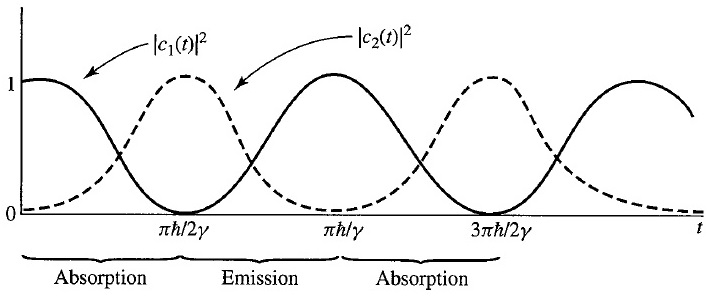
\includegraphics[width = 10cm]{./Graph/5.4.jpg}
\caption{当恰好处于共振$\omega=\omega_{21}$和$\Omega=\gamma/\hbar$时$|c_1(t)|^2$和$|c_2(t)|^2$关于$t$的图象。这一图像也体现了$|1\rangle$和$|2\rangle$间的相互变换。}
\label {Figure 5.4}
\end{centering}
\end{figure}

\

\noindent 这一吸收-发射循环过程即使在原理共振条件时也会出现。然而,$|2\rangle$的振荡振幅便会减小;$|c_2(t)|_{max}^2$不再是1,而且$|c_1(t)|^2$不再会降至0。在图5.5中我们将$|c_2(t)|_{max}^2$画成关于$\omega$的函数。这一曲线有一个以$\omega=\omega_{21}$为中心的共振波峰,且半峰宽度为$4\gamma/\hbar$。值得注意的是含时势强度越小($\gamma$越小),共振波峰越窄。

\begin{figure}
\begin{centering}
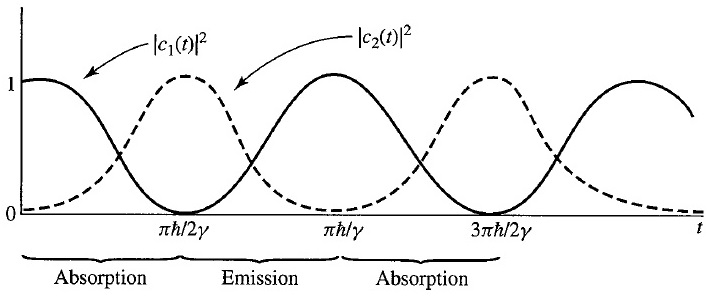
\includegraphics[width = 10cm]{./Graph/5.4.jpg}
\caption{$|c_2(t)|_{max}^2$关于$\omega$的图象,其中$\omega=\omega_{21}$对应于共振频率。}
\label {Figure 5.5}
\end{centering}
\end{figure}

\

\noindent \textbf{自旋磁共振}

\noindent 由(\ref{5.5.18})所定义的双态问题有很多的物理应用。作为第一个例子,考虑一个自旋为$\frac{1}{2}$的系统,在此假设是一个束缚电子,被置入一个不依赖于\emph{$t$}的$z$方向固定磁场,\emph{并且},外加一个在$xy$平面中旋转的依赖于\emph{$t$}的磁场:

\begin{equation} \label{5.5.26}
\boldsymbol{B}=B_0\hat{\boldsymbol{z}}+B_1(\hat{\boldsymbol{x}}\cos\omega t+\hat{\boldsymbol{y}}\sin\omega t)
\end{equation}

\noindent 其中$B_0$和$B_1$时常数。我们可以将不依赖于\emph{$t$}的固定磁场的效果表示为$H_0$并将旋转磁场的效果表示为$V$。由

\begin{equation} \label{5.5.27}
\boldsymbol{\mu}=\dfrac{e}{m_e c}\boldsymbol{S}
\end{equation}

\noindent 我们有

\begin{equation} \label{5.5.28}
\begin{split}
H_0=&\left(\dfrac{e\hbar B_0}{2m_e c}\right)(|+\rangle\langle+|-|-\rangle\langle-|)\\
V(t)=&\left(\dfrac{e\hbar B_1}{2m_e c}\right)[\cos\omega t(|+\rangle\langle-|+|-\rangle\langle+|)\\
&+\sin\omega t(-i|+\rangle\langle-|+i|-\rangle\langle+|)]\text{,}
\end{split}
\end{equation}

\noindent 其中我们用到了$2S_j/\hbar$的左右矢形式[见(\ref{3.2.1})]。对于$e<0$,$E_+$拥有比$E_-$更高的能量,而且我们发现可以用

\begin{equation} \label{5.5.29}
\begin{split}
|+\rangle\rightarrow|2\rangle\phantom{a}(\text{上能级})\\
|-\rangle\rightarrow|1\rangle\phantom{a}(\text{下能级})
\end{split}
\end{equation}

\noindent 来与(\ref{5.5.18})中的标记进行对照。这一双态系统的特征角频率为

\begin{equation} \label{5.5.30}
\omega_{21}=\dfrac{|e|B_0}{m_e c}\text{,}
\end{equation}

\noindent 也就是已在2.1节中考虑过的$B_0\neq0$,$B_1=0$问题的自旋进动频率。虽然$\langle S_{x,y}\rangle$的期望值由于逆时针方向(由正$z$轴方向看)的自旋进动而变化,$|c_+|^2$和$|c_-|^2$在不存在旋转场时却保持不变。我们现在引入一个由旋转场导致的新性质:$|c_+|^2$和$|c_-|^2$以关于$t$的函数形式来改变。这可以通过标识

\begin{equation} \label{5.5.31}
\dfrac{-e\hbar B_1}{2m_e c}\rightarrow\gamma\text{,}\omega\rightarrow\omega
\end{equation}

\noindent 来与(\ref{5.5.18})中的标记进行对照;我们的含时相互作用(\ref{5.5.28})恰好是(\ref{5.5.18})的形式。事实上$|c_+(t)|^2$和$|c_-(t)|^2$以$\omega=\omega_{21}$时图5.4中的方式进行变化而且按照(\ref{5.5.29})进行对应,比如,相当于自旋$\frac{1}{2}$系统经历了自旋反转的演替,$|+\rangle\Leftrightarrow|-\rangle$,以及自旋进动。半经典地来看,这一类的自旋反转可以被看做是由旋转$\boldsymbol{B}$体现的驱动转矩而导致的。

只要旋转磁场的频率与固定磁场的强度所决定的自旋进动频率恰好一致便可达到共振条件。我们可以看到自旋反转的概率相当大。

实际应用中,一个旋转磁场可能很难被人为生成。幸运的是,一个水平方向振荡的磁场,假设说,是在$x$方向上,就已经足够了。为了证明这一点,我们首先意识到这样一种振荡场可以被分解为一个逆时针分量和一个顺时针分量如下:

\begin{equation} \label{5.5.32}
2B_1\hat{\boldsymbol{x}}\cos\omega t=B_1(\hat{\boldsymbol{x}}\cos\omega t+\hat{\boldsymbol{y}}\sin\omega t)+B_1(\hat{\boldsymbol{x}}\cos\omega t-\hat{\boldsymbol{y}}\sin\omega t)
\end{equation}

\noindent 我们可以简单的通过翻转$\omega$的符号来得到逆时针方向分量的效果。假设逆时针分量符合共振条件

\begin{equation} \label{5.5.33}
\omega\simeq\omega_{21}
\end{equation}

\noindent 在一个典型的实验条件,

\begin{equation} \label{5.5.34}
\dfrac{B_1}{B_0}\ll 1\text{,}
\end{equation}

\noindent 也就是,由(\ref{5.5.30})和(\ref{5.5.31}),有

\begin{equation} \label{5.5.35}
\dfrac{\gamma}{\hbar}\ll\omega_{21}\text{;}
\end{equation}

\noindent 因此,只要逆时针分量符合共振条件,顺时针分量的效果便可以完全忽略,因为它相当于$\omega\rightarrow-\omega$,而且振幅的大小变得非常小并且很快的振荡。

我们现在求解的共振问题是解释原子、分子束和核磁共振实验的重要基础。通过变化振荡场的频率,我们可以非常准确的测量磁矩。我们这里的讨论基于微分方程组(\ref{5.5.17})的解;这个问题可以,甚至更优雅地,通过引入Rabi,Schwinger,和Van Vleck的旋转轴表示来求解。

\noindent \textbf{微波激射}

\noindent 作为另一个含时双态问题的应用示例,我们来考虑\textbf{微波激射}。特别地,我们来考虑一个氨分子$NH_3$,正如4.2节中所说的那样,它有两个相近的宇称本征态$|S\rangle$和$|S\rangle$且$|A\rangle$轻微得更高一点。令$\mu_{e\!l}$来表示分子的电偶极算符。出于对称性的考虑我们希望$\mu_{e\!l}$正比于$\boldsymbol{x}$,即$N$ 原子的位矢算符。基础相互作用为$-\mu_{e\!l}\cdot\boldsymbol{E}$,其中对于微波激射,$\boldsymbol{E}$是一个微波共振腔中的含时电场:

\begin{equation} \label{5.5.36}
\boldsymbol{E}=|\boldsymbol{E}|_{max}\hat{\boldsymbol{z}}\cos\omega t\text{。}
\end{equation}

\noindent 忽略$\boldsymbol{E}$的空间变化是合理的因为微波区域中的波长远大于分子的尺寸。频率$\omega$与$|A\rangle$和$|S\rangle$间的能量差相协调:

\begin{equation} \label{5.5.37}
\omega\simeq\dfrac{E_A-E_S}{\hbar}\text{。}
\end{equation}

\noindent 偶极算符的对角矩阵元由于宇称全部为零:

\begin{equation} \label{5.5.38}
\langle A|\mu_{e\!l}|A\rangle=\langle S|\mu_{e\!l}|S\rangle=0\text{,}
\end{equation}

\noindent 但是非对角元,一般来说,是不为零的:

\begin{equation} \label{5.5.39}
\langle S|\boldsymbol{x}|A\rangle=\langle A|\boldsymbol{x}|S\rangle\neq0\text{。}
\end{equation}

\noindent 这意味着存在一个含时势联系着$|S\rangle$和$|A\rangle$,并且我们早先讨论的双态问题现在便可以应用了。

我们现在便需要讨论微波激射是如何工作的。给定一个包含$|S\rangle$和$|A\rangle$的$NH_3$分子束,我们首先让分子束通过一个不含时非匀强电场区域来消除$|S\rangle$分量。这种电场可以用与Stern-Gerlach实验中的非均匀磁场将$|+\rangle$ 从$|-\rangle$分离的同种手段将$|S\rangle$从$|A\rangle$分离。$|A\rangle$的纯束接下来便进入一个与能量差$E_A-E_S$ 协调的微波共振腔。腔体的尺寸恰好令分子通过的时间为$(\pi/2)\hbar/\gamma$。这样一来我们便可以维持在图5.4的第一个发射相内;进入的是$|A\rangle$而出来的是$|S\rangle$。$|A\rangle$的激发能量在$|A\rangle$变为$|S\rangle$的过程中释放到含时势中继而令辐射(微波)场获得了能量。我们便通过辐射的受激发射,或者说是微波激射,来放大了微波。

实际上还有其他很多含时双态问题的应用实例,比如原子钟和光学抽运。实际上,可以有趣的看到多达有4次诺贝尔物理学奖都被颁给了那些探索某种形式含时双态系统的人。

\subsection{极端条件的含时哈密顿量}

\

\noindent 这一节致力于了解那些极快或极慢依赖于时间的含时哈密顿量的问题并给出一些“显然的”近似。我们仔细的观察,思考,指出一些有意思的现象,相关研究直到20世纪才逐渐清晰起来。

我们这里的方法局限于讨论一些基础,并给出一些特例。一个值得介绍但在此不讨论的例子就是方势阱阱壁的收缩或扩张,其中阱壁可以很快或很慢的运动。对于这一问题,我们建议有兴趣的读者参考D.N.Prinder,\emph{Am.J.Phys}\phantom{.}\textbf{58}(1990)54,以及D.W.Schlitt和C.Stutz,\emph{Am.J.Phys}\phantom{.}\textbf{38}(1970)70。

\noindent \textbf{瞬时近似}

\noindent 如果一个哈密顿量变化得太快,那么系统“没有时间”对变化进行调整。这使得系统处于与变化发生前相同的态中,同时这也是所谓“瞬时近似”的本质所在。

当然,虽然系统事先可能处于本征态,但我们没有理由相信它依旧是变化后哈密顿量的本征态。这提供了很有意思的物理机遇。一个典型的例子就是计算氚原子在$\beta$衰变后产生的$^3He^+$离子电子终态的显现情况。见本章末尾的问题5.35。

我们先来考虑瞬时近似的一个更精确的表述并给出一些结论。将时间演化算符的薛定谔方程(\ref{2.1.25})改写成

\begin{equation} \label{5.6.1}
i\dfrac{\partial}{\partial s}\mathcal{U}(t,t_0)=\dfrac{H}{\hbar/T}\mathcal{U}(t,t_0)=\dfrac{H}{\hbar\Omega}\mathcal{U}(t,t_0)\text{,}
\end{equation}

\noindent 其中我们将时间$t=sT$表示为与一个无量纲参数$s$和一个时间标度$T$有关,并且定义$\Omega\equiv1/T$。在瞬时近似中,时间标度$T\rightarrow0$,这意味着$\hbar\omega$比起$H$所代表的能量标度要大得多。假设我们可以通过添加或减掉一个任意常数来重定义$H$,在态矢中引入一些全局相因子,我们发现

\begin{equation} \label{5.6.2}
\mathcal{U}(t,t_0)\rightarrow1 \phantom{a}\text{当}T\rightarrow0
\end{equation}

\noindent 这证明了瞬时近似的有效性。这在$T$相比于$2\pi/\omega_{ab}$很小时应该是适当的,其中$E_{ab}=\hbar\omega_{ab}$ 是哈密顿量$H$两个相关的本征值之差。

\noindent \textbf{绝热近似}

\noindent 我们实际上往往会用绝热近似。给定一个依赖于某些参数组的哈密顿量,我们将会得到依赖于这些参数值得能量本征值。如果参数随时间“缓慢”变化,那么能量本征值就应该随着参数本身变化而取到它应有的值。关键在于什么是我们所说的“缓慢”。以量子力学或者某些角度来看,我们大概想要的是参数变化在一个时间标度$T$上并且要远大于某些能量本征值之差$E_{ab}$所定义的$2\pi/\omega_{ab}=2\pi\hbar/E_{ab}$。

一个显然的经典例子是在地表附近的摆。摆在你爬山时会正常摆动,只是由于重力的减小使得周期缓慢正常,制药高度变化经历的时间比起摆的周期要长得多。如果氢原子置入的电场缓慢变化,那么能级也会根据5.2节中计算的斯塔克效应来一步步变化。

我们来从量子力学的角度来考虑绝热变化的数学描述。我们跟随Griffiths(2005)的处理方法并着重注意相位作为关于时间的函数的变化。我们将态按照顺序用序号$n$标记并假设没有简并度因此不用考虑态的顺序会在时间变化中交叉。我们的出发点本质上是(\ref{2.1.27}),但是我们取$t_0=0$并舍弃初始时间的角标。

我们首先用标识写出本征值方程

\begin{equation} \label{5.6.3}
H(t)|n;t\rangle=E_n(t)|n;t\rangle\text{,}
\end{equation}

\noindent 注意到在任一时间$t$,态和本征值都可能改变。如果我们尝试寻找薛定谔方程

\begin{equation} \label{5.6.4}
i\hbar\dfrac{\partial}{\partial t}|\alpha;t\rangle=H(t)|\alpha;t\rangle
\end{equation}

\noindent 的通解,我们可以写出

\begin{equation} \label{5.6.5}
|\alpha;t\rangle=\displaystyle\sum_n c_n(t)e^{i\theta_n(t)}|n;t\rangle\text{,}
\end{equation}

\noindent 其中
\begin{equation}\label{5.6.6}
\theta_n(t)\equiv-\dfrac{1}{\hbar}\displaystyle\int_0^t E_n(t')dt'\text{。}
\end{equation}

\noindent 将展开系数拆分为因子$c_n(t)$和$\exp(i\theta_n(t))$在之后会被验证是很有意义的。将(\ref{5.6.5})代入(\ref{5.6.4})并用(\ref{5.6.3}),我们得到

\begin{equation} \label{5.6.7}
\displaystyle\sum_n e^{i\theta_n(t)}\left[\dot{c}_n(t)|n;t\rangle+c_n(t)\dfrac{\partial}{\partial t}|n;t\rangle\right]=0\text{。}
\end{equation}

\noindent 现在,用$\langle m;t|$取内积并考虑同时间的本征态正交归一,我们便可得到关于$c_n(t)$的微分方程,也就是

\begin{equation} \label{5.6.8}
\dot{c}_m(t)=-\displaystyle\sum_n c_n(t) e^{i[\theta_n(t)-\theta_m(t)]}\langle m;t|\left[\dfrac{\partial}{\partial t}|n;t\rangle\right]\text{。}
\end{equation}

内积$\langle m;t|(\partial/\partial t)|n;t\rangle$是一个新的特性。如果$H$是不依赖时间的,那么$|n;t\rangle$将是定态,通常的自然常数的含时幂也会显现出来。为了更广义的来看这一问题,我们可以回到(\ref{5.6.3})并对两边求时间导数。对于$m\neq n$的情况,我们有

\begin{equation} \label{5.6.9}
\langle m;t|\dot{H}|n;t\rangle=[E_n(t)-E_m(t)]\langle m;t|\left[\dfrac{\partial}{\partial t}|n;t\rangle\right] \text{。}
\end{equation}

\noindent 这使得我们可以将(\ref{5.6.8})重写为

\begin{equation} \label{5.6.10}
\dot{c}_m(t)=-c_m(t)\langle m;t|\left[\dfrac{\partial}{\partial t}|m;t\rangle\right]-\displaystyle\sum_n c_n(t)e^{i(\theta_n-\theta_m)}\dfrac{\langle m;t|\dot{H}|n;t\rangle}{E_n-E_m}\text{,}
\end{equation}

\noindent 







\end{document}
